\chapter{BPELRF}\label{chapter:c3}
\markboth{Chapter~\ref{chapter:c3}. Design and Verification of Web Service Compositions}{}
%
%This chapter presents a methodology called \textit{Correct-WS} for the creation of correct Web Service compositions including time constraints. Some of the model translations needed among the different phases of this methodology are described in detail and a tool that we have developed to automate these translations of the methodology is also introduced. Next, a case study showing a Web Service composition for an Internet purchase process is presented, where the tool is applied for the development of a correct composition. Finally, the remaining translations of the methodology and other parallel works are briefly referenced.
%
%\section{Correct Web Services Methodology}\label{Correct-WS}
%\markright{~\ref{Correct-WS} Correct Web Services Methodology}
%
%The \textit{Correct Web Services Methodology} or \textit{Correct-WS} for short is a methodology that can be used for the design and implementation of correct Web Services \cite{Cambronero2007}. We consider that a Web Service is correct if it is well designed, that is, it has been checked for potential design errors. These errors can be specific, i.e., errors that are checked via properties that are specific to the current application, or general, i.e., errors related to general characteristics of software systems such as concurrency, quality of service, time response, security, \ldots
%
%It is necessary to apply a methodology covering every phase of the life cycle for the generation of Web Service compositions, as in the generation of other software applications. In Figure \ref{TopDownDesign} we can see a diagram showing a schematic view of the \textit{Correct-WS} methodology. It consists of the following phases:
%
%\begin{figure}[h]
%\begin{center}
%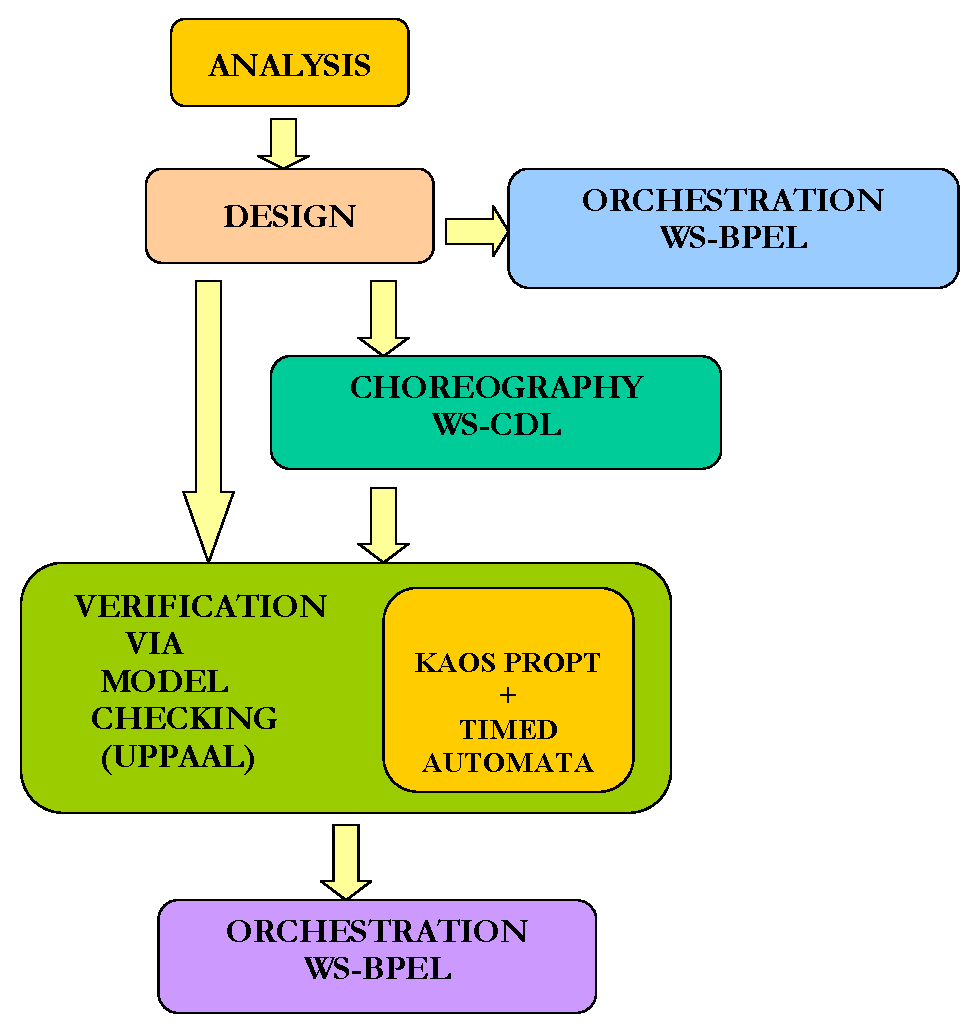
\psfig{file=Figures/topdownlast.eps,scale=.55}
%\end{center}
%\caption{Scheme of the \textit{Correct-WS} methodology.}
%\label{TopDownDesign}
%\end{figure}
%
%\begin{enumerate}
%
%\item \textbf{Analysis phase}: In the analysis phase it is used a technology based on goal models performing requirement engineering called KAOS \cite{Lamsweerde1993} in order to capture the requirements that the system must fulfil.
%
%\item \textbf{Design phase}: In the design phase we use Unified Modeling Language (UML) 2.0 sequence diagrams in order to design the system behaviour in a proper way \cite{OMG2003}.
%
%\item \textbf{Verification of the design phase}: The UML 2.0  sequence diagrams representing Web Service compositions with time constraints are translated into timed automata, in order to verify properties on it by using UPPAAL tool. The properties to check are those that we have established in the analysis phase. If we detect some failures here, then we can correct them in an earlier phase. In this way, we can reduce future failures in the system.
%
%\item \textbf{Choreography implementation phase}: It is done automatically the translation of the verified UML 2.0  sequence diagrams into the choreography layer document written in WS-CDL. The same process can be performed for WS-BPEL.
%
%\item \textbf{Verification of choreography implementation phase}: The generated WS-CDL documents are translated into timed automata, since during the implementation phase some new failures can appear in the system. Then the UPPAAL tool verifier is used again in order to check and correct failures, going back to the second step if some failures are found.
%
%\item \textbf{Verification of orchestration implementation phase}: The enriched obtained WS-BPEL documents are translated into timed automata, and we can recheck properties on it. If a failure is detected, the procedure is the same than in the fifth step. The  WS-BPEL document can also be obtained from the corresponding timed automata document.
%
%\end{enumerate}
%
%In Figure \ref{methosteps} we can see a schematic view of the translations included in the \textit{Correct-WS} methodology.
%
%\begin{figure}[h]
%\begin{center}
%\psfig{file=Figures/Methodologysteps.eps,scale=.60}
%\end{center}
%\caption{Translations included in the Correct-WS Methodology.}
%\label{methosteps}
%\end{figure}
%
%The main activity in the performance of the goal-oriented requirements engineering in the \textbf{analysis phase} is the construction of the goal model. Goals are objectives the system under construction must achieve, that is, the properties that the system must fulfil. Goals can be formulated at different levels of abstraction, from high-level strategic concerns to low-level technical concerns, and it is possible the definition of alternative refinements for a given goal.
%
%The structure of the goal model is an AND/OR graph, being the KAOS methodology the specific goal-oriented framework considered here \cite{Lamsweerde1993}. This methodology considers a two level language: (i) an outer semi-formal layer for capturing requirements engineering concepts, structuring and presenting them, and (ii) an inner formal assertion layer for the precise definition of the requirements and for reasoning about them. The different parties cooperating for the achievement of a goal are called \textit{agents}. They are active components that play a role towards goal satisfaction. The goals can refer to the provided services (functional goals) or to the quality of these services (non-funtcional goals).
%
%In KAOS the goals that build goal models are organized in AND/OR refinement-abstraction hierarchies where higher-level goals are usually strategic, coarse-grained and involve multiple agents, whereas lower-level goals are usually technical, fine-grained and involve fewer agents. The AND-refinement links relate a goal to a set of subgoals possibly conjoined with domain properties, that is, satisfying all subgoals in the refinement is a sufficient condition in the domain for satisfying the goal. The OR-refinement links relate a goal to a set of alternative subgoals. In Figure \ref{AndRefinementOrRefinement} we can see an AND-refinement on the left-hand side and an OR-refinement on the right-hand side .
%
%\begin{figure}[h]
%\begin{center}
%\psfig{file=Figures/AndRefinement.eps,scale=.70}
%\psfig{file=Figures/OrRefinement.eps,scale=.70}
%\end{center}
%\caption{AND-refinement and OR-refinement goal models.}
%\label{AndRefinementOrRefinement}
%\end{figure}
%
%The goals of the goal model in KAOS can be formalized in a real-time temporal logic like the one supported by the UPPAAL tool. According to the temporal behaviour pattern they prescribe, goals are considered of type \textit{achieve} (reachability), \textit{maintain} (safety), possibly always, inevitably and unbounded response. The correspondence between these different kinds of goals and their graphical representation is depicted in Table \ref{tablareqeriments}.
%
%\begin{table}
%\begin{center}
%
%\begin{tabular}[t]{|p{5.5cm}|c|}
%  \hline
%  % after \\: \hline or \cline{col1-col2} \cline{col3-col4} ...
%  \textbf{Temporal Behaviour} & \textbf{Goal Model Representation} \\
%  \hline
%  Maintain (Safety) $A$[ ] $\varphi$ & \includegraphics[width=5cm]{Figures/Maintain.eps}  \\
%  \hline
%  Achieve (Reachability) $E<> \varphi$ & \includegraphics[width=5cm]{Figures/Achieve.eps} \\
%  \hline
%  Possibly Always $E$[ ] $\varphi$ & \includegraphics[width=5cm]{Figures/PossiblyAlways.eps} \\
%  \hline
%  Inevitably $A<> \varphi$ & \includegraphics[width=5cm]{Figures/Inevitably.eps} \\
%  \hline
%  Unbounded Response $\varphi --> \psi$ & \includegraphics[width=5cm]{Figures/UnboundedResponse.eps} \\
%  \hline
%\end{tabular}
%\caption{KAOS requirements goal model representation.}
%\label{tablareqeriments} 
%\end{center}
%\end{table}
%
%The \textbf{design phase} is aimed at the system description in order to capture each particular behaviour in the system. In particular, we are interested in Unified Modeling Language (UML) 2.0  sequence diagrams because they can represent the message flow and the behaviour of several processes including time constraints.
%
%Next section shows in detail the use of UML  2.0  sequence diagrams in the design phase and the translation rules of these diagrams into WS-CDL specifications in order to get automatically these choreography documents from a model of the system (fourth phase of the \textit{Correct-WS} methodology).
%
%\section{Translation of UML 2.0 Sequence Diagrams into WS-CDL}\label{UML2WSCDL}
%\markright{~\ref{UML2WSCDL} Translation of UML 2.0 Sequence Diagrams into WS-CDL}
%
%Our starting point is a UML 2.0 sequence diagram extended with frames \cite{Ambler2005}. A frame is defined as a unit of behaviour and contains, among others, related objects and the sequence of messages between these objects. A frame is depicted by a solid-outline rectangle with a pentagon in the upper left corner name-label, which makes it easier to refer to it, for example as a subdiagram.
%
%The following specific frames are considered in the translation (Figure \ref{figuraframes}):
%
%\begin{figure}[h]
%\begin{center}
%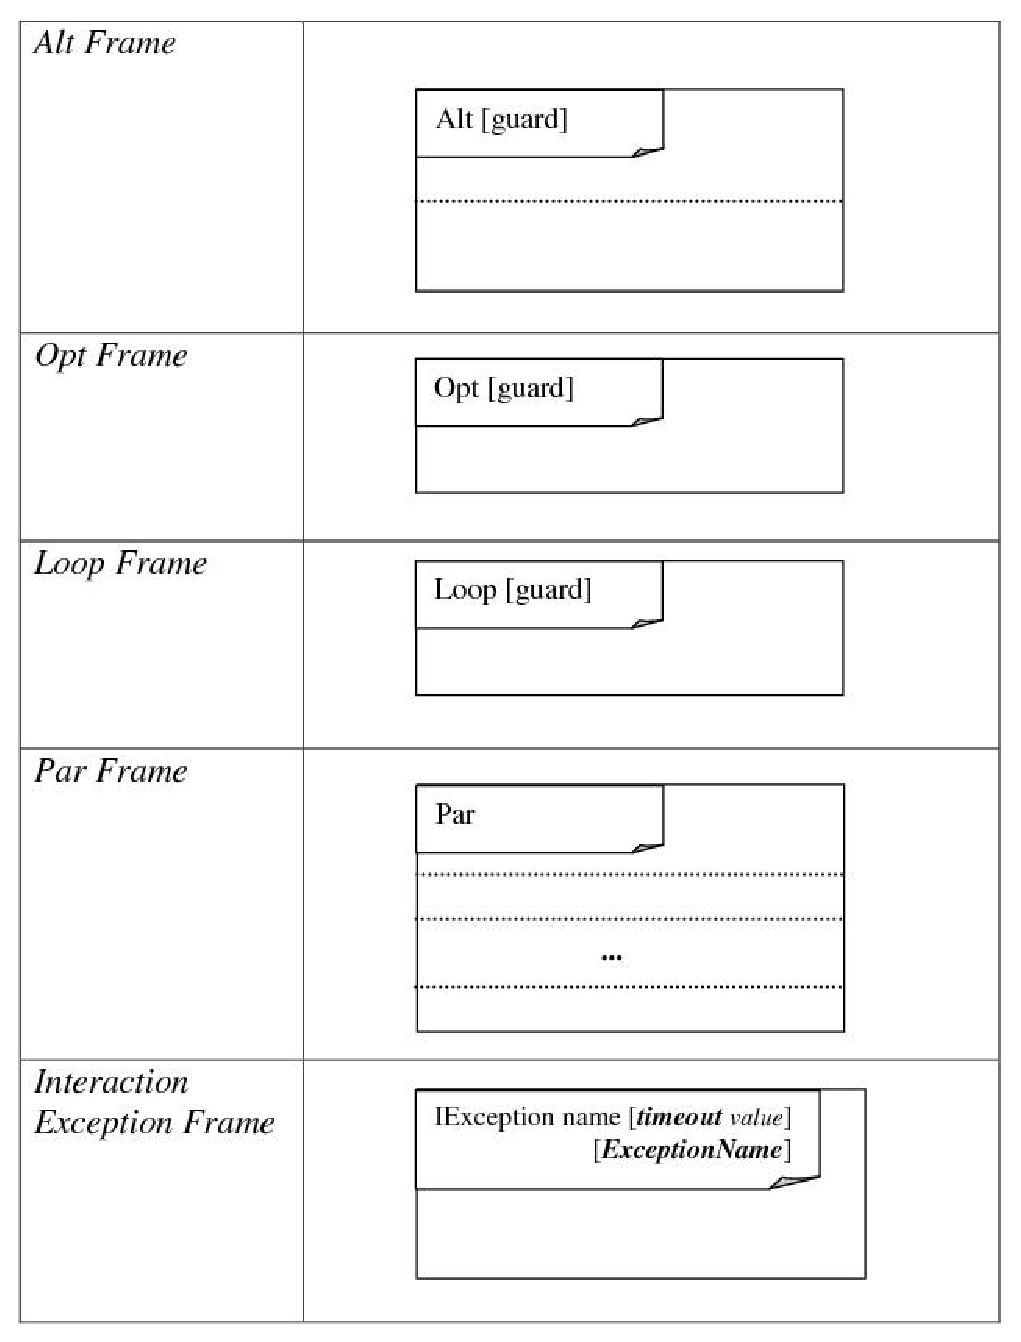
\psfig{file=Figures/Frames.eps,scale=.60}
%\end{center}
%\caption{UML 2.0 frames considered in the model.}
%\label{figuraframes}
%\end{figure}
%
%\begin{itemize} 
%
%\item {\em Alt-labelled frames}: These frames allow us to specify an {\em if-then-else} control structure, depending on a condition that follows the {\em alt} label. There is also a version of this frame without condition in which the choice is non-deterministic.
%
%\item {\em Opt-labelled frames}: These frames allow us to specify an {\em if-then} control structure, depending on the condition that follows the {\em opt} label.
%
%\item {\em Loop-labelled frames}: These frames allow us to describe a repetitive behaviour, depending on the repetition condition that follows the {\em loop} label.
%
%\item {\em Par-labelled frames}: These frames are use to describe parallel message exchange activities.
%
%\item {\em Interaction exception frames}: These frames are associated with interactions and express fault conditions. They are pictured as separated frames, linked by an arrow to the interaction they are associated with. It should be noted that an interaction may have an associated time out, so a specific type of interaction exception frame is considered in this case.
%
%\end{itemize}
%
%\begin{figure}[h]
%\begin{center}
%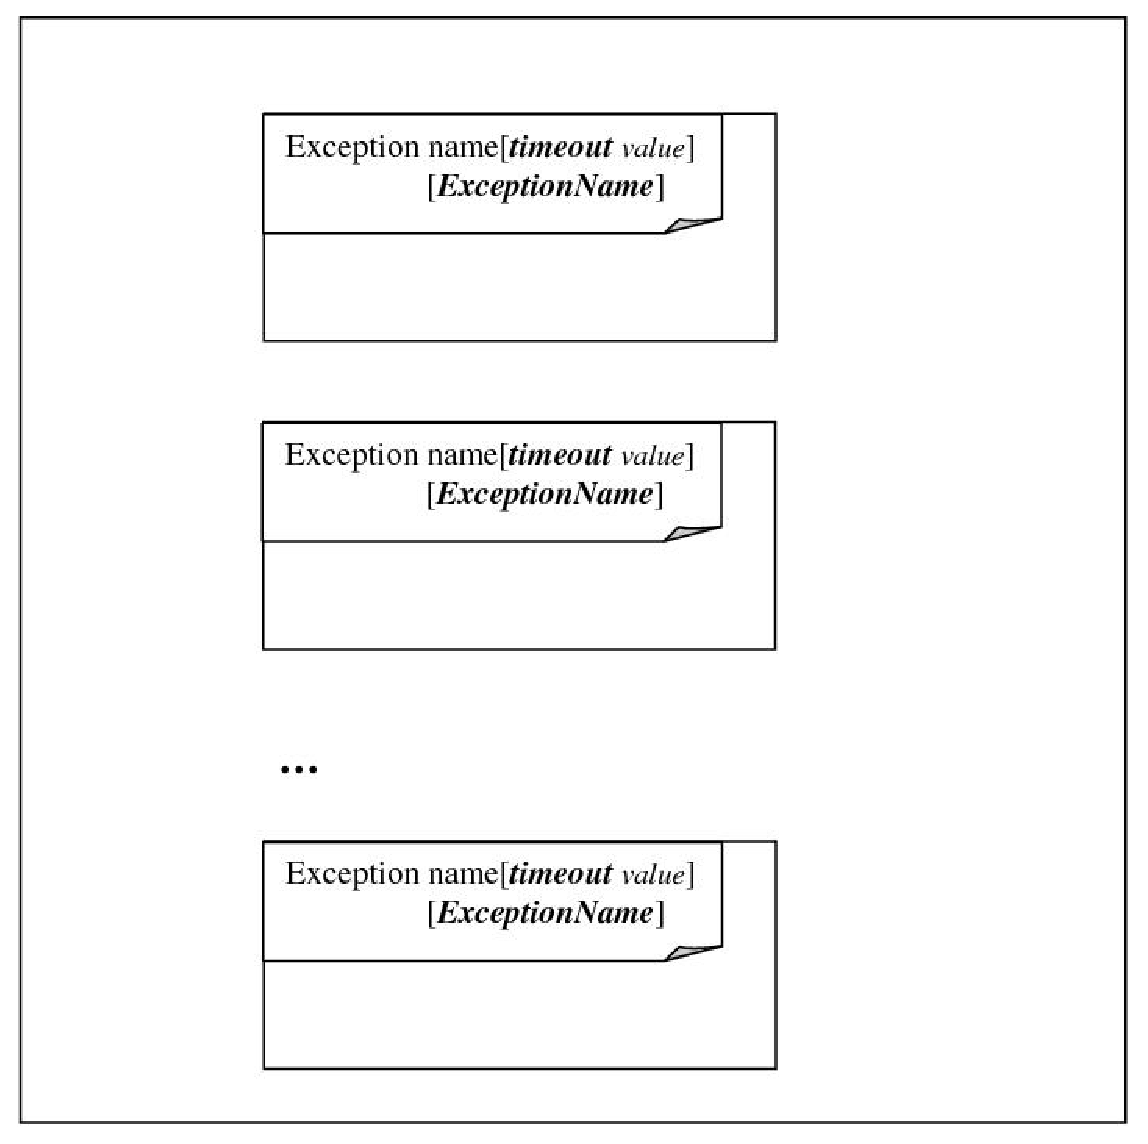
\psfig{file=Figures/exceptionframes.eps,scale=.60}
%\end{center}
%\caption{Structure of an exception sequence diagram.}
%\label{FramesException}
%\end{figure}
%
%Together with the sequence diagram capturing the main control flow, there is a so-called {\em exception sequence diagram}, which consists of a set of {\em Exception frames}, one for each interaction fault condition (Figure \ref{FramesException}). Each {\em Exception frame} is labelled with the corresponding interaction fault condition and only comes into play when this specific error has occurred.
%
%Frames are therefore a powerful tool to describe the control structure of a Web Service composition, as well as the exceptional situations that may arise when two parties interact. Furthermore, we can use frame conditions to specify constraints that can include a wide range of information, such as expressions using variables, clocks, etc. As a result, frame-extended UML 2.0 allows us to describe Web Service compositions with time restrictions.
%
%Once the UML sequence diagrams with the appropriate frame extension have been introduced, the translation can be described, which is made on a structural basis, that is, the translation for each element in the frame-extended UML 2.0 sequence diagrams is provided (Tables \ref{esquema-tradu} and \ref{framesUW}): 
%
%\begin{table}
%\begin{center}
%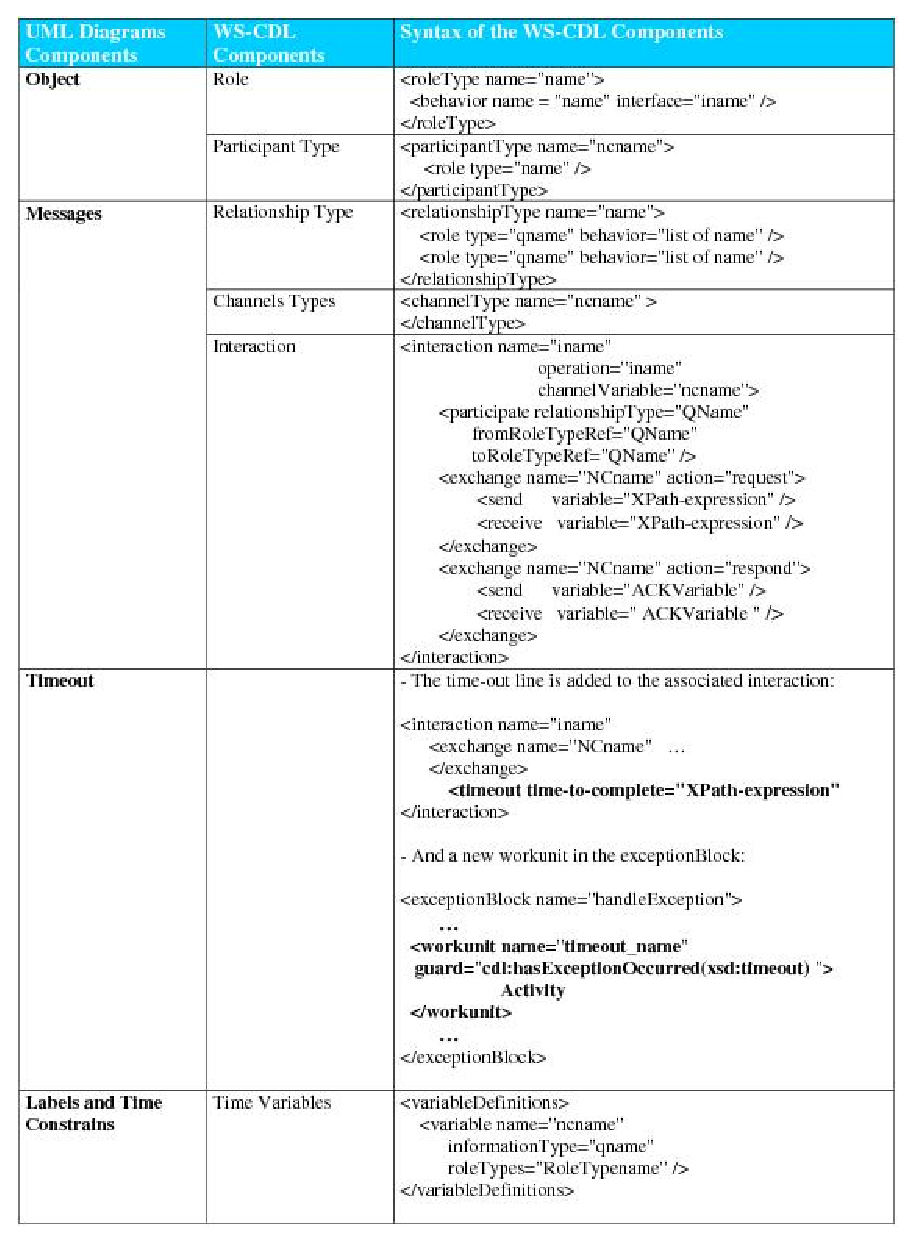
\psfig{file=Figures/tablaUMLCDL1.eps,scale=.85}
%\end{center}
%\caption{Translation of UML 2.0 sequence diagram elements into WS-CDL.}
%\label{esquema-tradu}
%\end{table}
%
%\begin{table}
%\begin{center}
%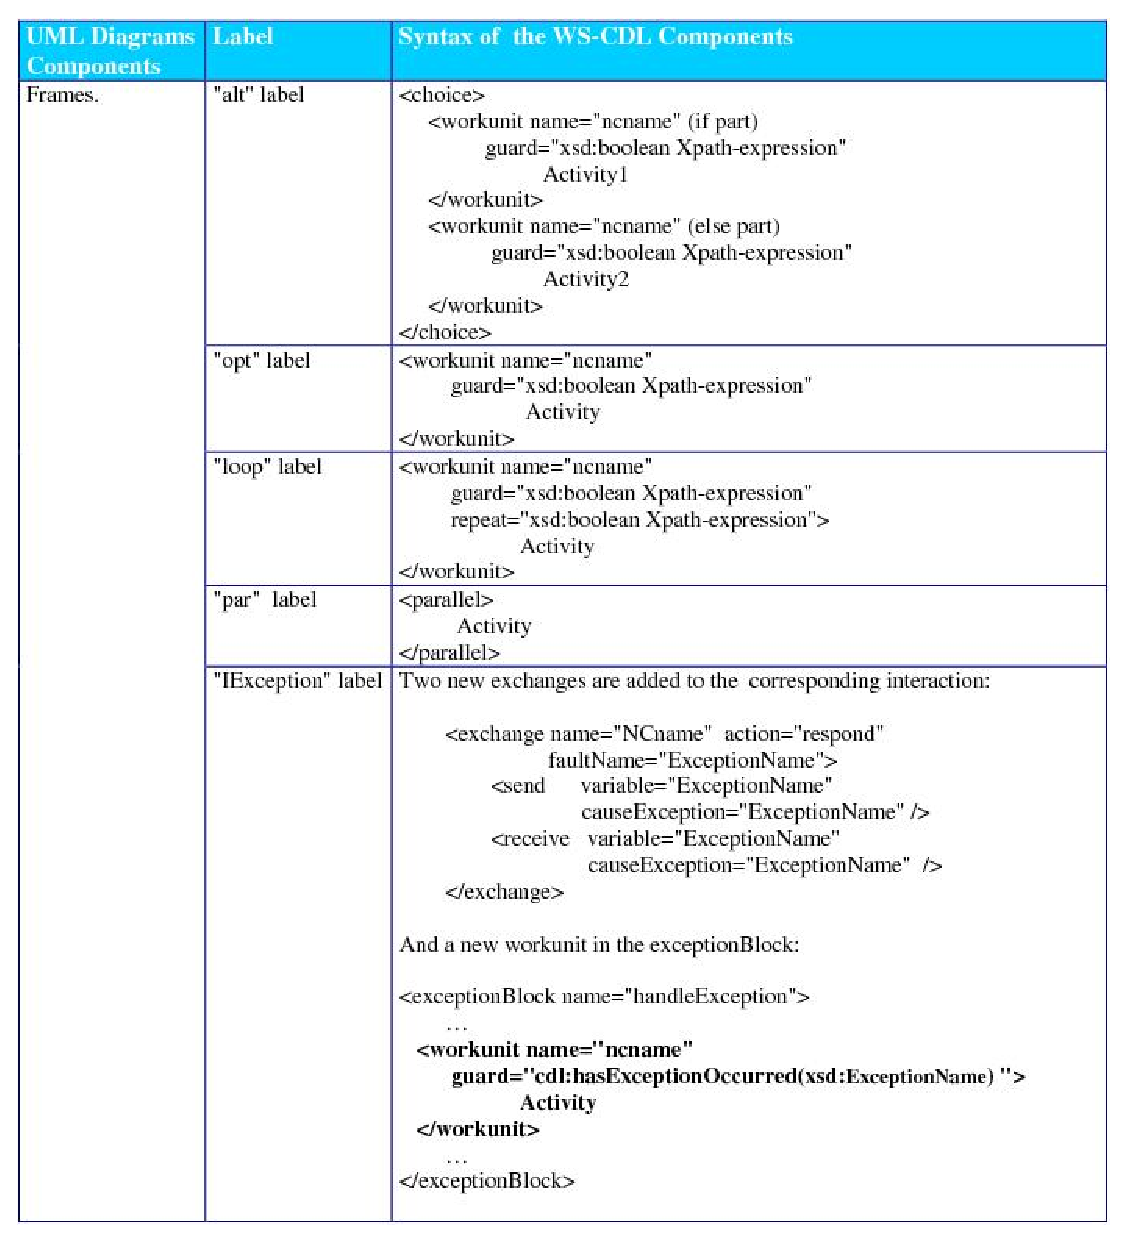
\psfig{file=Figures/tablaUML-WSCDL11.eps,scale=.70}
%\end{center}
%\caption{Translation of UML 2.0 frames into WS-CDL.}
%\label{framesUW}
%\end{table}
%
%\begin{itemize}
%
%\item \emph{Objects}: The objects in the UML 2.0 sequence diagrams correspond to the WS-CDL role types, which are used to describe the behaviour of each class of party involved in the choreography. Each object is then translated into a different WS-CDL role type. We also consider a participant type for the object with its associated role type.
%
%\item \emph{Messages}: Each message in the UML 2.0 sequence diagram is translated as a WS-CDL interaction with a {\em Request} exchange element followed by a {\em Respond} exchange element. For this purpose, it is also needed to declare a new {\em channel type}, as well as a new {\em relationship type}. The channel type declares the channel used for the communication and
%the relationship type specifies the two role types (objects) involved in this interaction, which has a {\em Request-exchange} element, corresponding to the sending of the message specified in the UML sequence diagram, as well as a {\em Respond-exchange} element capturing the message {\em ack} in the case of successful transmission. Furthermore, as it is shown later, if this transmission has an associated time out or any other interaction exception frame, these fault conditions will enrich the  interaction syntax by adding elements to it.
%
%\item \emph{Variables}, \emph{expressions} and \emph{time constraints}: These elements are translated into WS-CDL information types, variables and expressions in XPath \cite{W3C1999}. From the UML 2.0 sequence diagram we obtain the corresponding {\em Information types} for the WS-CDL translation. These are the same types of variables used in the UML sequence diagram. Each variable is then translated into a WS-CDL variable (with the same name), using the corresponding information type. Time constraints are translated into XPath expressions with the appropriate XPath operators.
%
%\item \emph{Par-labelled frames}: These frames are translated as \textit{parallel} ordering structures, indicating the activities running in parallel.
%
%\item \emph{Loop-labelled frames}: These frames are translated into WS-CDL \textit{workunits}, indicating iterative computations. The loop condition (expressed in XPath) is thus used both for the workunit guard and for its repetitive behaviour.
%
%\item \emph{Opt-labelled frames}: These frames are also translated as \textit{workunits}. In this case, the Boolean expression following the keyword {\em opt} is used as the guard for the workunit.
%
%\item \emph{Alt-labelled frames}: These frames are translated using a {\em choice} ordering structure and two guarded workunits as alternatives. The Boolean expression following the keyword {\em alt} is now used as a guard for the first workunit, whose actions are taken from the activities inside the {\em then}-part of the frame, whereas the guard of the second workunit is the negation of that condition. According to WS-CDL semantics, only the workunit in which the guard is evaluated to true will be performed. The version of this frame without condition is also translated using a {\em choice} ordering structure, but in this case without workunits inside, so the choice is non-deterministic.
%
%\item {\em Interaction exception frames}: These frames are translated by adding new elements to the interaction they are associated with. Two cases can be distinguished:
%
%\begin{itemize}
%
%\item {\em Timeout}: When the transmission of a message has an associated time out, a time out element is included in the associated interaction. 
%              
%\item \emph{Others}: For any other interaction exception frame a new {\em Respond-exchange} element is considered within the associated interaction, with the {\em faultName} attribute, which is used to indicate that this exchange corresponds to a failure, and also the {\em causeException} attribute must be included in both the {\em send} and the {\em receive} parts of the exchange, indicating the thrown exception.
%     
%\end{itemize}
%
%\item {\em Exception frames}: The exception frames within the {\em Exception sequence diagram} are translated into WS-CDL using the {\em choreography exception block}, in which there are as many exception workunits as exception types. An exception workunit is a guarded workunit, in which the {\em hasExceptionOccurred} WS-CDL function is used to check the exception that has been thrown. Thus, only the corresponding exception workunit is performed.
%
%\end{itemize}
%
%Next section is about the translation of the generated WS-CDL documents into timed automata for validation and verification of the choreography implementation (fifth phase of the \textit{Correct-WS} methodology).
%
%\section{Translation of WS-CDL Documents into Timed Automata}\label{WSCDL2TA}
%\markright{~\ref{WSCDL2TA} Translation of WS-CDL Documents into Timed Automata}
%
%The obtained WS-CDL specification is translated into a network of timed automata (NTA) that allows us to validate and verify the expected requirements of the system. In the timed automata model that we consider there are non-negative integer variables and urgent edges. The variables can be assigned a value when executing an edge, and their values can be checked in the guards and invariants. Urgent edges inhibit time elapsing when they are enabled.
%
%A function ~\mbox{$\varphi$} is first defined which associates an NTA to every WS-CDL activity, where ~\mbox{$\varphi:{\it Activities} \times {\cal P}_{\cal F}(C) \times {\cal N} \longrightarrow {\it NTA} \times  {\cal P}_{\cal F}(C)$}. The main argument of this function is the activity for which the translation is made, but it has two additional arguments: one set of clocks (${\cal P}_{\cal F}(C)$) and one location (${\cal N}$). The set of clocks must be reset just before finishing the execution of the generated timed automata (for compositional purposes). The location is used to transfer the control flow there in the event of a failure. This location is used as an argument in order to link the normal activity flow with the exception part.
%
%The first projection of $\varphi$ is denoted by $\varphi_1(A,C,l)$, that is, the obtained NTA, and its second projection by $\varphi_2(A,C,l)$, that is, the set of clocks that should be reset when using this NTA compositionally.
%
%A choreography is now defined as a pair $(A_1,\{A_{2_{i}}\}_{i \in I})$, where $A_1$ is the activity of the choreography {\it life-line}\,,and $\{A_{2_{i}}\}_{i \in I}$ is the set of exception workunits of its exception block, which can be empty (denoted by $\emptyset$), because the exception block is optional.
%
%Thus, given a choreography $\mathcal{C}=(A_1,\{A_{2_{i}}\}_{i \in I})$, its associated NTA is defined as follows (Figure \ref{NTA1}):
%
%\begin{figure}[h]
%\begin{center}
%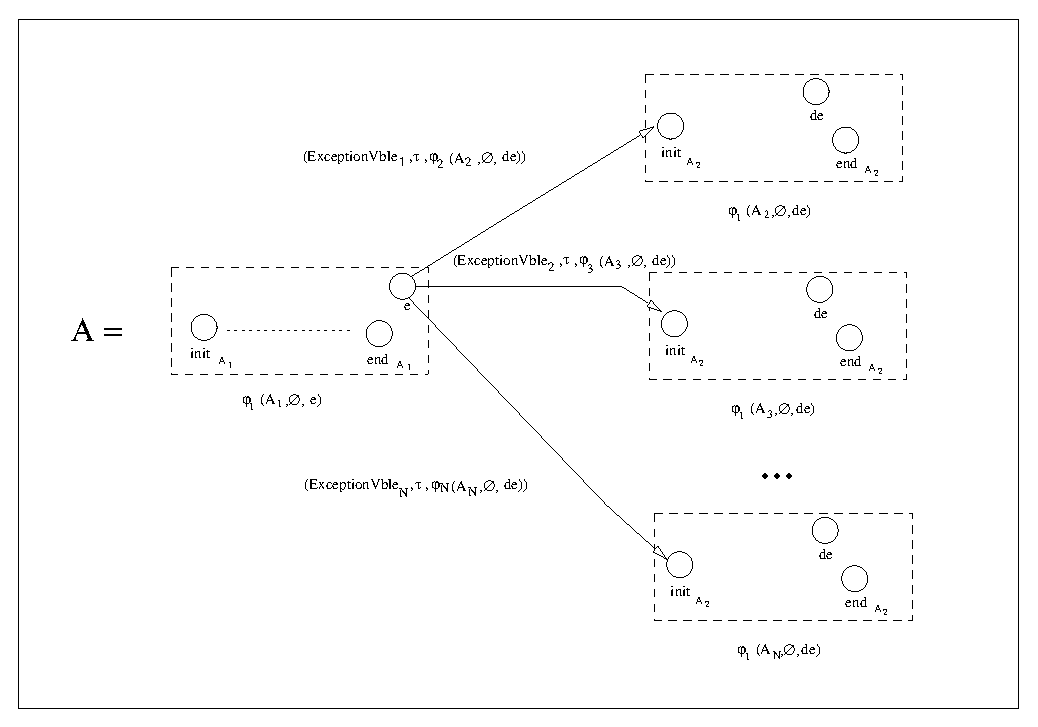
\psfig{file=Figures/choreography.eps,scale=.80}
%\end{center}
%\caption{From WS-CDL to NTA (I).}
%\label{NTA1}
%\end{figure}
%
%\begin{itemize}
%
%\item It is first created a location `{\it de}', which is called the ``double exception location''. It is used as the location to which the control flow is transferred in the event of a failure within an exception activity $A_{2_{i}}$. It is then generated $\varphi(A_{2_{i}},\emptyset,{\it de})$, for $i \in I$.
%
%\item It is created the exception location `{\it e}', to which the control flow is transferred in the event of failure in $A_1$, and then we generate $\varphi(A_1,\emptyset,e)$.
%
%\item The exception location `{\it e}' is connected with the initial locations of the NTAs corresponding to the exception workunits, according to the exception thrown, by means of urgent edges, which must reset all the clocks in $\varphi_2(A_{2_{i}},\emptyset,{\it de})$, with $i \in I$. As can be seen in Figure \ref{NTA1}, urgent edges are graphically distinguished by a white arrowhead and are given the highest priority when enabled.
%
%\end{itemize}
%
%Figures \ref{NTA2} and \ref{NTA3} show how the function $\varphi$ is defined for the different activities of WS-CDL. It can be seen that all the obtained automata have both one initial and one final location, this property being preserved by all the constructions. In the event of a failure, all of these constructions transfer the control flow to the location indicated as parameter in the function $\varphi$, and reset the clocks indicated as parameters in all the edges reaching the final location.
%
%\begin{figure}
%\begin{center}
%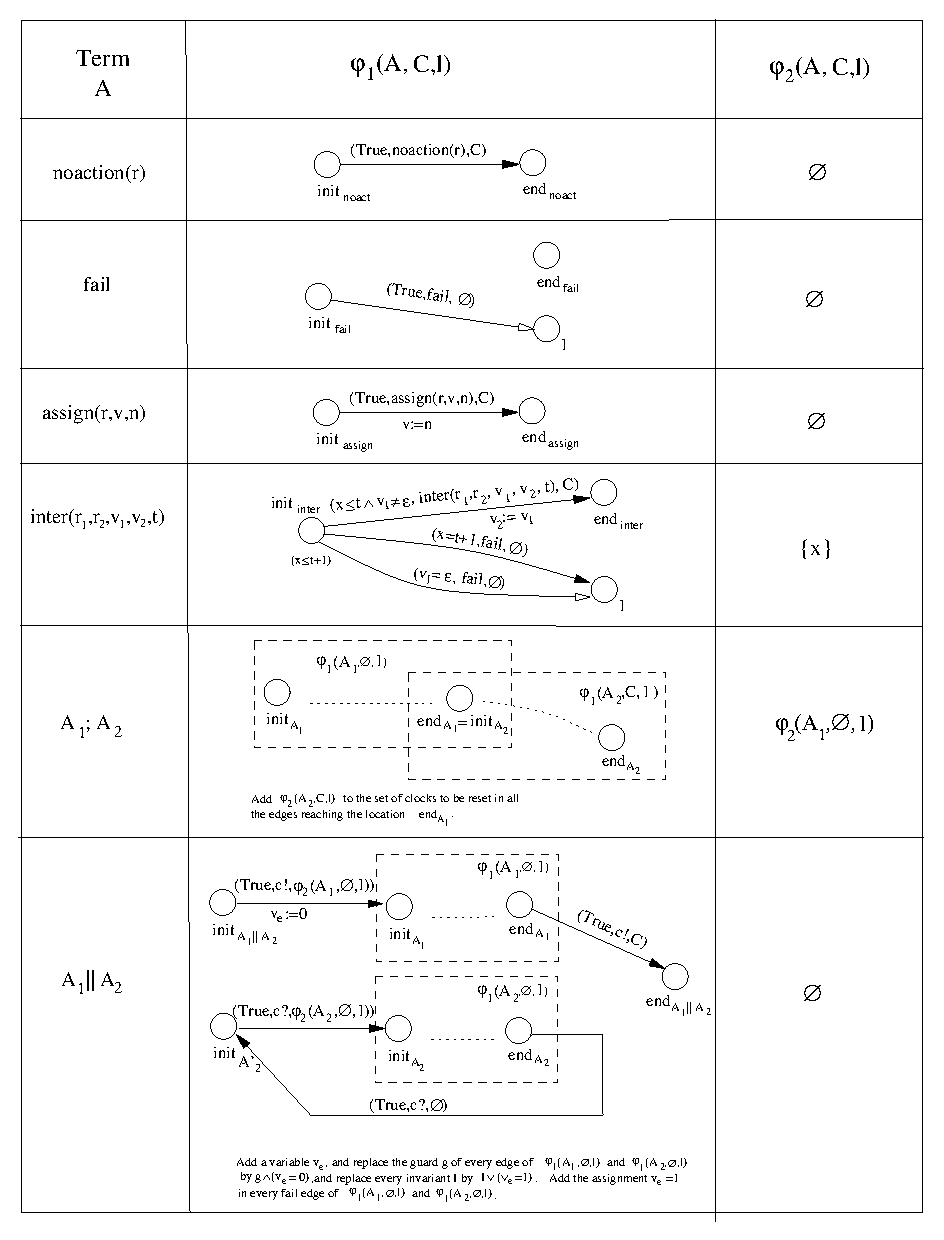
\psfig{file=Figures/wscdl2ta1.eps,scale=.90}
%\end{center}
%\caption{From WS-CDL to NTA (II).}
%\label{NTA2}
%\end{figure}
%
%\begin{figure}
%\begin{center}
%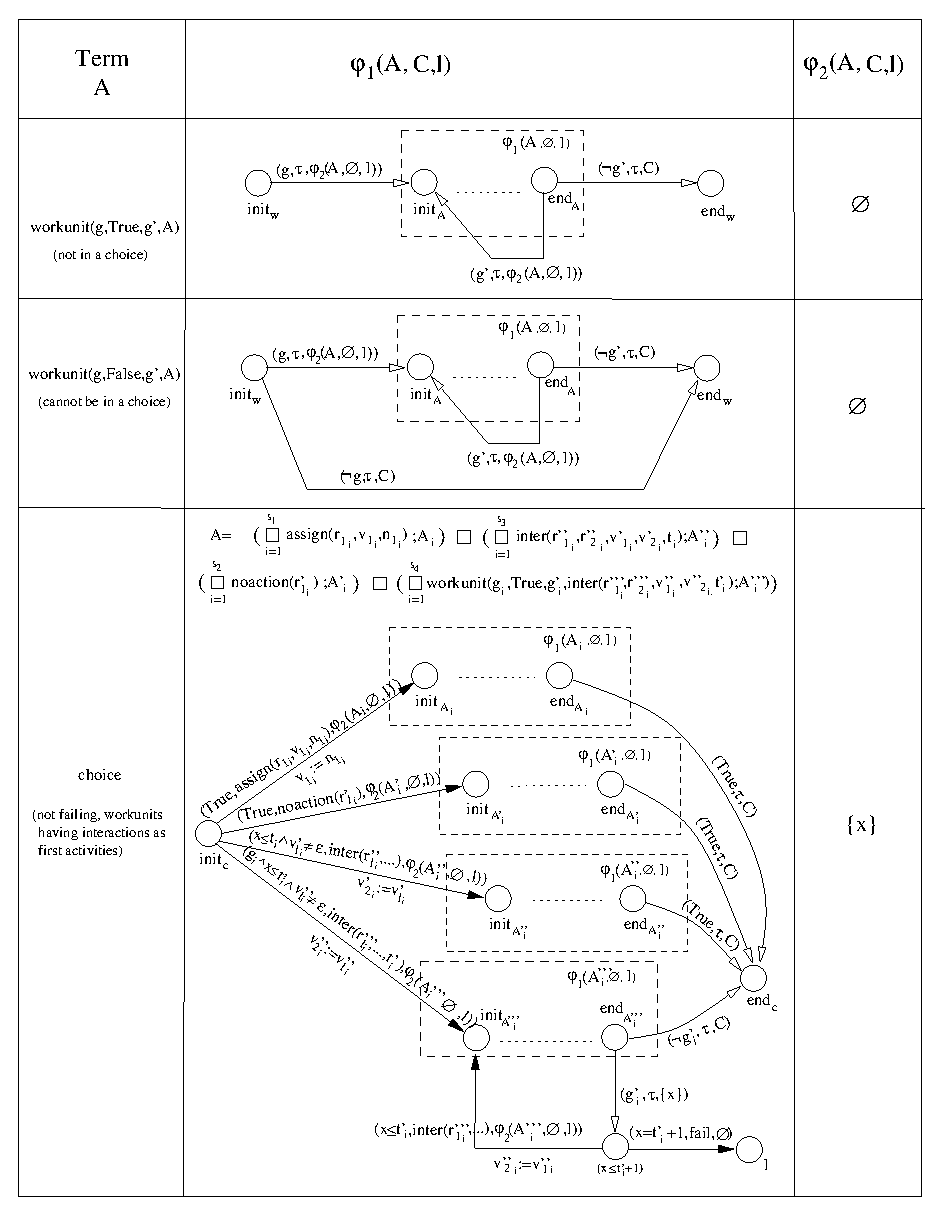
\psfig{file=Figures/wscdl2ta2.eps,scale=.90}
%\end{center}
%\caption{From WS-CDL to NTA (III).}
%\label{NTA3}
%\end{figure}
%
%Let us now describe how the translation works for the different activities:
%
%\begin{itemize}
%
%\item \textbf{noaction}, \textbf{fail} and \textbf{assign}: these activities have a simple translation, as we only have to introduce an edge connecting the initial location with the final one (the exception location in the case of {\em fail}). In the case of the {\em noaction}\, activity, it captures either a silent or internal operation at role $r$. Notice that in the case of {\em fail}, the edge is urgent, since no time can elapse when a fail action can be executed. The {\it assign} activity is used to assign the variable $v$ at role $r$ to $n$, and in this case we can observe that we need to introduce the corresponding assignment operation in the timed automaton.
%
%\item \textbf{interaction}: we consider an interaction $inter$ between roles $r_1$ and $r_2$, with a time out $t$ (which can be infinite), where the value of variable $v_2$ in $r_2$ is assigned to the value of variable $v_1$ of $r_1$. In this case three edges must be considered, one for the interaction execution, which must be performed within the indicated time interval, and only when $v_1$ has a value assigned, and two additional edges to capture the two possible cases of failure: time out expiration (captured by using a location invariant) and $v_1$ unassigned (this edge must be urgent). Notice that when $t=\infty$ the time out edge would not be introduced.
%
%\item \textbf{sequence}: in the case of a sequence of two activities $A_1$ and $A_2$, denoted as $\mathbf{ \,\,A_1 \,; A_2 \,\,}$, we first obtain the corresponding NTA both for $A_1$ and $A_2$, as indicated in Figure \ref{NTA2}, and then we only need to collapse in a single location the final node of $\varphi_1(A_1,\emptyset,l)$ and the initial node of $\varphi_1(A_2,C,l)$. Notice that all the edges reaching this node must reset all the clocks in $\varphi_2(A_2,C,l)$, and also that the set of clocks to be reset when using the generated NTA is that of $A_1$.
%
%\item \textbf{parallel}: in the case of a parallel execution of two activities $A_1$ and $A_2$, denoted as $\mathbf{ \;A_1 \,\| \, A_2 \,\,}$, we first obtain the corresponding NTA both for $A_1$ and $A_2$, and then we add three new locations and the edges indicated in Figure \ref{NTA2} needed to enforce the simultaneous initialization and termination of both activities, by means of a new synchronization channel $c$. We also add a new variable $v_e$, initialized to 0, which is used to prevent the execution of further transitions of one of the automata when the other one has failed. Thus, we add the guard condition $(v_e=0)$ to every edge of both automata, and also the invariants $I$ are replaced by $(I \vee v_e=1)$, to avoid the time lock of the system when a {\em fail} has been executed. Furthermore, the assignment $v_e=1$ is now included in every {\em fail} edge of both automata.
%
%\item \textbf{workunit}: The workunit activity has the following interpretation: firstly, if some of the variables used in guard condition $g$ are not available, or if $g$ evaluates to false then, depending on the value of {\em block}\, attribute (\emph{True} or \emph{False}), the workunit is skipped or it is blocked until $g$ is evaluated to true. When the guard evaluates to true, the activity $A$ inside the workunit is executed, and when it terminates the repetition condition $g'$ is evaluated. If some variable used in $g'$ is not available or if $g'$ is false, the workunit terminates, otherwise the activity inside is executed again. In the translation of this activity we have distinguished two cases depending on the {\em block} value, as indicated in Figure \ref{NTA3}, the difference being that when {\em block} is false there is an urgent edge connecting the new initial location with the new final location, labelled with the action $\tau$, which resets the clocks in $C$. Notice that in both cases if $g$ is evaluated to true, the control flow is immediately transferred to the initial location of $\varphi_1(A,\emptyset,l)$ by means of another urgent edge, and also that upon termination of $A$ the repetition guard $g'$ is immediately checked in order to decide whether $A$ should be repeated or the control should be transferred to the new final location.
%
%\item \textbf{Choice}: The choice operator has a semantics that allows any alternative to proceed by executing any of its enabled actions, which generates some problems in the translation, especially in the case of workunits as alternatives of a choice. We have previously imposed the restriction for these workunits that are alternatives of a choice to have their block argument equals to true, but we need to impose some additional restrictions on them in order to define this translation. The first additional restriction that we consider is that their first activity must be an interaction (it would not be problematic to assume that this activity is either a {\em noaction} or an {\em assign}, but in such a case the translation would be slightly different). We also impose that no parallel activity appears as alternative in a choice, to avoid a rather large distinction of subcases. Then, to simplify the description this case is not considered. With these assumptions we define the translation for the choice operator by unfolding all the inner choices it can contain, i.e., we define the translation
%for a {\em general choice}\, in which we may have as alternatives the following activities: {\em assign}, {\em noaction}, {\em inter} and {\em workunit}, possibly in a sequence with any other operator. Figure \ref{NTA3} shows how this translation is made
%for a general choice in which we have all of these activities as alternatives. However, notice that a choice can also {\em fail}, but only in the case that all the alternatives  {\em fail}. This means, for instance, that if we have either an {\em assign} or a {\em noaction} as one alternative of the choice, no {\em fail} action is possible. Then, in the case of a choice with no {\em assign} and no {\em noaction} as alternatives, we must consider the two possible cases of failure: either the maximum time-out $M$ of all the alternative interactions has expired, with $M = {\it Max}(t_1,\ldots,t_{s_{3}},t'_1,\ldots,t'_{s_{4}})$, or no source variable of these interactions has a value assigned. In Figure \ref{NTA4} we depict the two urgent edges that we should add in this case\footnote{If $M=\infty$ the time-out edge would not appear.}. Finally, we have omitted any consideration to the case in which the {\em fail} activity is an alternative of the choice, because this {\em fail} action could not ever be executed, so it could be removed.
%
%\begin{figure}[h]
%\begin{center}
%\psfig{file=Figures/failtaprueba.eps,scale=.95}
%\end{center}
%\caption{Fail Edges in a Choice.}
%\label{NTA4}
%\end{figure}
%
%\end{itemize}
%
%As a result of this translation, an NTA representing the behaviour of the Web Service composition is obtained. This NTA representation can be directly used in the UPPAAL tool, to carry out simulations and also to verify the properties that were identified in the analysis phase.
%
%In next section we describe the tool that we are developing to automate some phases of the \textit{Correct-WS} methodology called  Web Service Translation tool, WST for short.
%
%\section{Web Services Translation Tool (WST)}\label{WST}
%\markright{~\ref{WST} Web Services Translation Tool (WST)}
%
%Web Services Translation Tool (WST) is an integrated environment for translating XMI documents \cite{OMG1998} corresponding to UML 2.0 sequence diagrams into WS-CDL specifications and WS-CDL specifications into timed automata supported by the UPPAAL tool. WST has been developed in Java and the tool, its source code and some documentation is available at http://www.dsi.uclm.es/retics/WST/\,.
%
%WST applies several XSLT Stylesheets \cite{W3C1999-2} to an initial XML document to obtain a new XML document. For instance, four XSL Stylesheets are used in order to translate an initial WS-CDL document into another XML document representing the timed automata system supported by the UPPAAL tool. XSLT and other related standards are described in detail in Appendix \ref{a1}.
%
%The tool is divided into three different tabs, allowing the user to perform different tasks: the design of a UML 2.0 sequence diagrams and the exportation of these diagrams to XMI documents, the translation of the XMI documents into WS-CDL specifications, and the translation of WS-CDL specifications into XML documents describing timed automata supported by the UPPAAL tool.
%
%In the next subsections each one of these tabs composing the WST tool is described in more detail.
%
%\subsection{UML 2.0 Sequence Diagram Editor}\label{WST_Editor}
%
%The first tab of the WST tool allows the user to model an UML 2.0 sequence diagram representing the interactions between the different parties in the composition and including time restrictions. A diagram showing the different parts of this editor is shown in Figure \ref{CapturaEditor}.
%
%\begin{figure}[h]
%\begin{center}
%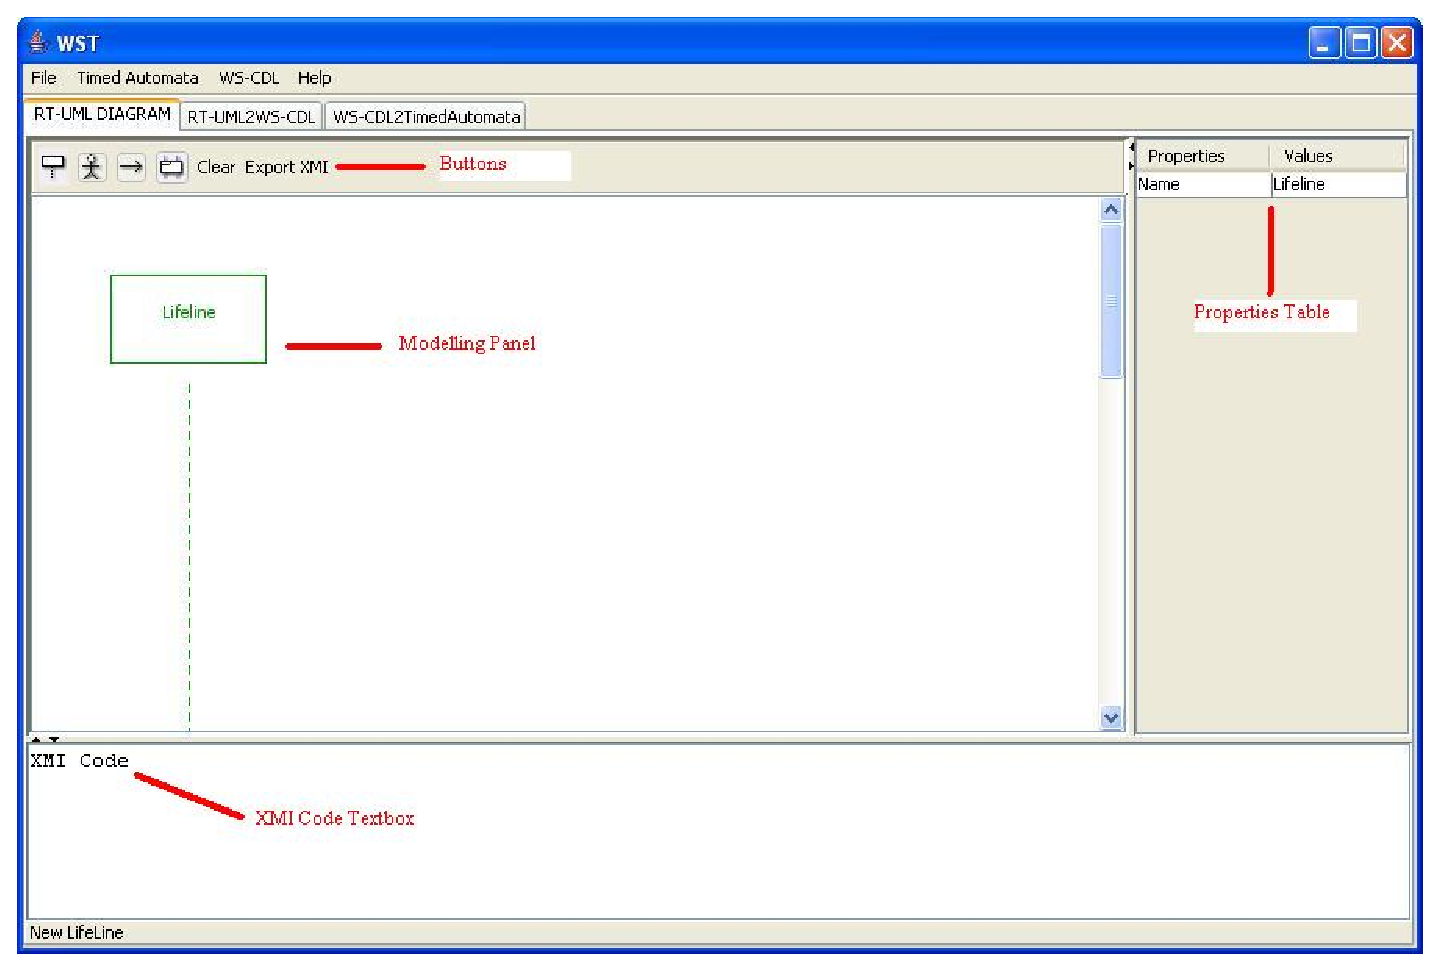
\psfig{file=Figures/captura.eps,scale=.60}
%\end{center}
%\caption{UML 2.0 sequence diagram editor of WST.}
%\label{CapturaEditor}
%\end{figure}
%
%The \emph{Modelling Panel} has six buttons on the top, from left to right:
%
%\begin{itemize}
%    
%\item The \textbf{New Lifeline} button allows the user to include a new lifeline in the diagram. By left-clicking the button, the tool automatically includes the new lifeline after the actors and the lifelines included before with a default name (\textit{Lifeline}, \textit{Lifeline1}, \textit{Lifeline2}, \ldots).
%    
%\item The \textbf{New Actor} button allows the user to include a new actor in the diagram. By left-clicking the button, the tool automatically includes the new actor after the lifelines and actors included before with a default name (\textit{Actor}, \textit{Actor1}, \textit{Actor2}, \ldots).
%
%\item The \textbf{New Message} button allows the user to create a new message interaction between two different parties. The user must left-click over the first element on the panel (actor or lifeline sender of the message) and then left-click over the second element (actor or lifeline receiver of the message). After clicking both elements the tool will display a message from the first element to the second element with a default name (\textit{Message}, \textit{Message1}, \textit{Message2}, \ldots). The order of the message in the diagram relative to other messages and frames added before depends on the height where the user left-click over the first element, including the message as part of a frame if the user left-click inside the frame.
%
%\item The \textbf{New Frame} button allows the user to add a new frame to the diagram. By left-clicking the button, the user can choose the type of frame to create: \textit{Alt alternative}, \textit{Alt if/else}, \textit{Opt optional}, \textit{Loop}, \textit{Par parallel} or \textit{Exception}. After that, except in the case of the \textit{Exception} frame which is automatically place at the end of the diagram, the user must left-click over one actor or lifeline (it does not matter which one) to place the frame in the diagram. The order of the frame in the diagram relative to other messages and frames added before depends on the height where the user left-click over the diagram, including the frame as part of another frame if the user left-click inside this other frame.
%    
%\item The \textbf{Clear} button allows the user to delete the current diagram completely, starting the design again from scratch. By left-clicking the button, a dialog will be shown to the user to confirm the action of deleting all the components.
%    
%\item The \textbf{Export XMI} button allows the user to create an XMI document corresponding to the current diagram. By left-clicking the button, a dialog will be shown to the user to select the name and the place of this document in the operating system. Once the code has been saved, it will be display also in the \emph{XMI Code Textbox} of the tab.
%
%\end{itemize}
%
%The different types of frames that can be included in the diagram have the following meanings:
%
%\begin{itemize}
%
%\item \textbf{Alt alternative}: This frame is divided into different parts (from 2 to n) which meaning is that only one of this parts is executed but we do not now which one (we do not have any way to know which part will be chosen).
%
%\item \textbf{Alt if/else}: This frame is divided into two parts, the \textit{if} part and the \textit{else} part. It has a guard condition that determines which part is executed, the \textit{if} part if the guard is fulfilled and the \textit{else} part if the guard is not fulfilled.
%
%\item \textbf{Opt optional}: The content of this frame is executed only if its guard condition is fulfilled, otherwise the execution waits until the condition is fulfilled or skips the frame content and continues after it, depending on the definition of the guard as blocking or non-blocking.
%
%\item \textbf{Loop}: The content of this frame is executed repetitively while its repeat condition is fulfilled, finishing when the repeat condition is not fulfilled. It can also have a guard condition (optional) to start its execution and this condition can be blocking (the execution wait until the condition is fulfilled) or non-blocking (the execution skips the frame content and continues after it if the condition is not fulfilled).
%
%\item \textbf{Par parallel}: This frame is divided into different parts (from 2 to n) which meaning is that each part is executed in parallel with the other parts.
%
%\item \textbf{Exception}: The content of this frame is executed when its exception condition is thrown in the main workflow, finishing all the execution when the content of the frame is performed.
%
%\end{itemize}
%
%To save the diagram modelled, the user must choose the \textbf{Save UML Diagram...} option in the \textbf{File} menu. A dialog will be shown to the user to specify the name and the place where this diagram is saved in the operating system.
%
%To load a diagram previously saved, the user must choose the \textbf{Open UML Diagram...} option in the \textbf{File} menu. A dialog will be shown to the user to select the diagram to be opened. If the file opened is not a valid diagram, an error message will be displayed.
%
%In the following paragraphs it is described the edition options the users have over each type of component that can be included in the diagram.
%
%\textbf{\subsubsection{Lifeline and Actor Components}}
%
%Once the user has added a lifeline or an actor component to the diagram, it is possible to change the component name by double-clicking over it (its colour will change to orange). A text box will be shown to the user to edit the component name. This name cannot be repeated, otherwise an error message will be shown. Another way to change the component name is by modifying the value of the \textit{Name} field in the \emph{Properties Table} of the tab. The properties corresponding to a component will be shown in this table by left-clicking over the component (its colour will change to green). 
%
%By right-clicking over one of these components a drop down menu will appear showing two options, \textit{Delete} and \textit{Variables}. If the user selects the first option (the colour of this component and all other components affected will change to red) a dialog will be shown to confirm the action of deleting this component. If the user selects the second option a new dialog will be shown to manage variables associated with the object. This dialog allows the user to create variables (with type clock, integer, boolean, string or exception), assign initial values to this variables, if possible, and delete variables previously created. The variable names cannot be repeated.
%
%\textbf{\subsubsection{Message Components}}
%
%Once added a message to the diagram by the user, it is possible to change the component name by double-clicking over it (its colour will change to orange). A text box will be shown to the user to edit the component name. This name cannot be repeated, otherwise an error message will be shown. Another way to change the message name is by modifying the value of the \textit{Name} field in the \emph{Properties Table} of the tab. The properties corresponding to a message will be shown in this table by left-clicking over the component (its colour will change to green).
%
%By right-clicking over a message a drop down menu will appear showing five options: \textit{Delete}, \textit{Update variables}, \textit{Exchange variables}, \textit{Time to complete} and \textit{Cause exception}. If the user selects the first option (the message colour will change to red) a dialog will be shown to confirm the action of deleting this component. If the user selects the second option a new dialog will be shown to manage the updating of variables previously created. This dialog allows the user to update a variable value (with a valid value) and to delete updates previously created (removing the content of the value text field and pressing the update button). If the user selects the third option a new dialog will be shown to manage the exchange of variables previously created. The \textit{Send} variable text field is used to specify the variable sent and the \textit{Receive} variable text field is used to specify the variable in which the value of the sent variable is received. Both variables must have the same type. If the user selects the fourth option a new dialog will be shown to establish a time out. The user must specify the value of the time out and the clock name in this dialog. Finally, if the user selects the last option a new dialog will be shown to establish an exception that can be thrown by the interaction. This exception must be an exception variable previously defined.
%
%\textbf{\subsubsection{Frame Components}}
%
%By right-clicking over a frame (the colour of this component and all other components affected will change to red) a dialog will be shown to confirm the action of deleting this component. This is a general behaviour to all the different frame types but other behaviours depends on the frame type.
%
%Some frame types have guard expressions related with them. These expressions can have equality and inequality operators ($==$, $!=$) or relational operators ($<$, $<=$, $>=$, $>$), and can be combined by means of logical operators ($and$ and $or$). The variables used in the guards must be previously defined, otherwise an error message will be display.
%
%The edition options specific to each type of frame are the following:
%
%\begin{itemize}
%
%\item \textbf{Alt alternative}: This component has no properties to set up, so left-clicking or double-clicking over it have not effect.
%
%\item \textbf{Alt if/else}: This component has a guard to determine which part of the frame is executed. By double-clicking over this component it is possible to specify its guard expression. It is compulsory to set a guard for this frame before exporting the diagram to an XMI document. Another way to change the component guard is modifying the value of the \textit{Guard} field in the \emph{Properties Table} of the tab. The properties corresponding to this frame will be shown in this table by left-clicking over the component (its colour will change to green).
%
%\item \textbf{Opt optional}: This frame also has a guard to determine if its content is executed and this guard can be blocking or non-blocking. By double-clicking over this component it is possible to specify its guard expression and if the guard is or is not blocking. It is compulsory to set a guard for this frame before exporting the diagram to an XMI document. Another way to change the component guard and blocking behaviour is editing the value of the \textit{Guard} and \textit{Block} fields (respectively) in the \emph{Properties Table} of the tab. The properties corresponding to this frame will be shown in this table by left-clicking over the component (its colour will change to green).
%
%\item \textbf{Loop}: This frame has a repeat condition and its execution is repeated until this condition is not fulfilled (but the condition is tested at the end of the execution, so it has at least one execution). By double-clicking over this component it is possible to specify its repeat expression. It is compulsory to set a repeat expression for this frame before exporting the diagram to an XMI document. Another way to change the component repeat condition is modifying the value of the \textit{Repeat} field in the \emph{Properties Table} of the tab. This frame can also has a guard expression to start its execution and this expression can be blocking or non-blocking. By double-clicking over this component it is possible to specify its guard expression and if the guard is or is not blocking. This expression is optional so it is possible to export a diagram with this frame to an XMI document without specifying a guard value. In this case, no guard will be taken into account. Another way to change the component guard and blocking behaviour is editing the value of the \textit{Guard} and \textit{Block} fields (respectively) in the \emph{Properties Table} of the tab. The properties corresponding to this frame will be shown in this table by left-clicking over the component (its colour will change to green).
%
%\item \textbf{Par parallel}: This component has no properties to set up, so left-clicking or double-clicking over it have not effect.
%
%\item \textbf{Exception}: This frame has a name and an exception condition, and its execution is performed when the exception in the condition is thrown (an exception variable or a time out). By double-clicking over this component it is possible to specify its exception name and condition. It is compulsory to set an exception condition for this frame before exporting it to an XMI document. Another way to change the exception name and condition is modifying the value of the \textit{Name} and \textit{Exception} fields (respectively) in the \emph{Properties Table} of the tab. The properties corresponding to this frame will be shown in this table by left-clicking over the component (its colour will change to green).
%
%\end{itemize}
%
%\subsection{XMI to WS-CDL Translator}\label{WST_XMI2WSCDL}
%
%The second tab of the WST tool allows the user to transform the XMI code corresponding to a UML 2.0 sequence diagram (generated in the previous tab) into a WS-CDL specification. A diagram showing the different parts of this tab is shown in Figure \ref{CapturaXMI2WSCDL}.
%
%\begin{figure}[h]
%\begin{center}
%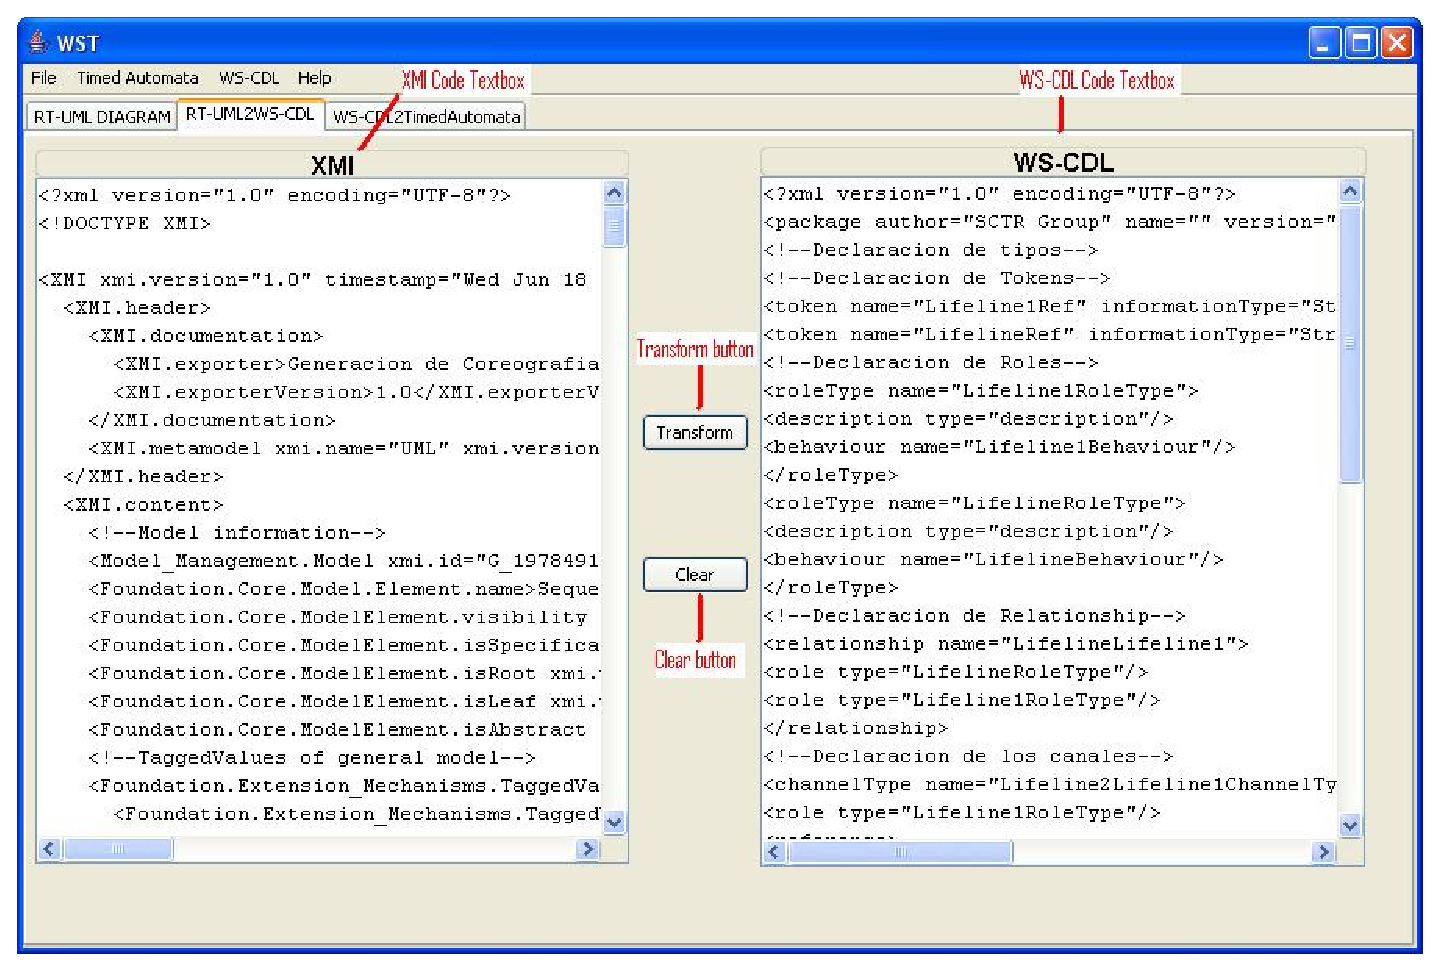
\psfig{file=Figures/captura2.eps,scale=.60}
%\end{center}
%\caption{XMI to WS-CDL translator of WST.}
%\label{CapturaXMI2WSCDL}
%\end{figure}
%
%In this tab the following elements can be distinguished:
%
%\begin{itemize}
%
%\item The \textbf{XMI Textbox} where the XMI code to transform is shown. This code will be loaded automatically when the sequence diagram is exported to an XMI file in the first tab. Another way to load the XMI code is using the \textbf{Open XMI File...} option in the \textbf{File} menu. A dialog will be shown to the user to select the code to be opened. If the file opened is not valid, an error message will be displayed on the screen.
%
%\item The \textbf{WS-CDL Textbox} where the WS-CDL specification will be shown after doing the transformation. To save the specification, the user must choose the \textbf{Save WS-CDL File...} option in the \textbf{WS-CDL} menu. A dialog will be shown to the user to specify the name and the place where this specification is saved in the operating system.
%
%\item The \textbf{Transform} button allows the user to generate the WS-CDL specification corresponding the XMI code loaded in the \textbf{XMI Textbox}. The result will be automatically displayed in the \textbf{WS-CDL Textbox} after a few seconds. If the \textbf{XMI Textbox} is empty pressing the Transform button will have no effect.
%
%\item The \textbf{Clear} button allows the user to clear the content of both, the \textbf{XMI Textbox} and the \textbf{WS-CDL Textbox}.
%
%\end{itemize}
%
%\subsection{WS-CDL to Timed Automata Translator}\label{WST_WSCDL2TA}
%
%The third tab of the WST tool allows the user to transform the WS-CDL specification (generated in the previous tab) into a network of timed automata that can be opened by the UPPAAL tool. A diagram showing the different parts of this tab is shown in Figure \ref{CapturaWSCDL2TA}.
%
%\begin{figure}[h]
%\begin{center}
%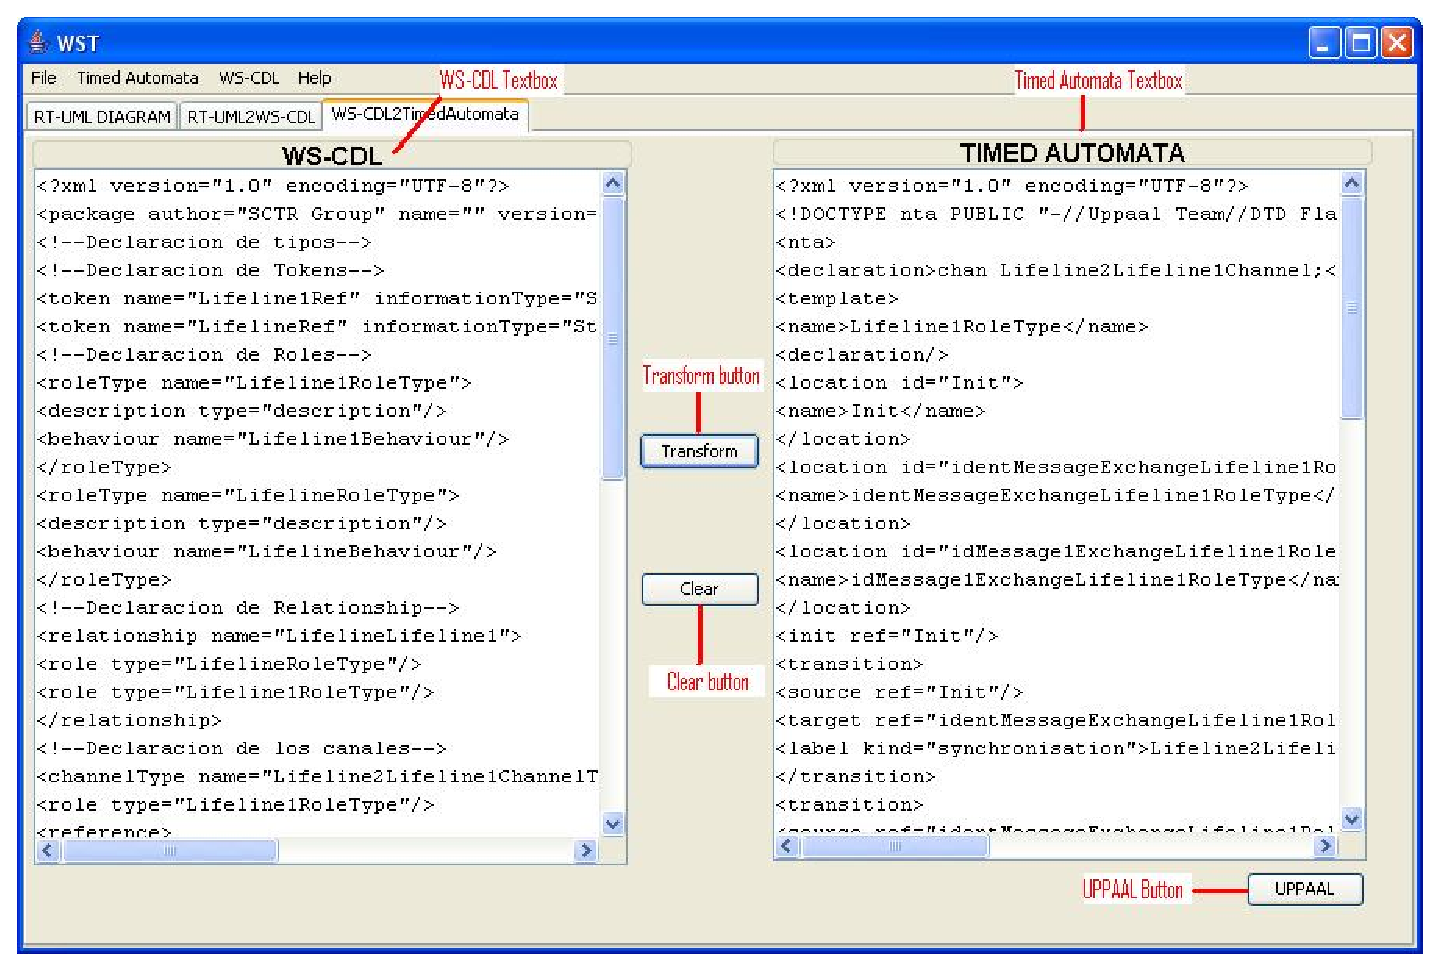
\psfig{file=Figures/captura3.eps,scale=.60}
%\end{center}
%\caption{WS-CDL to timed automata translator of WST.}
%\label{CapturaWSCDL2TA}
%\end{figure}
%
%In this tab the following elements can be distinguished:
%
%\begin{itemize}
%
%\item The \textbf{WS-CDL Textbox} where the WS-CDL specification to transform is shown. This specification will be loaded automatically when the WS-CDL specification generated in the previous tab is saved. Another way to load the WS-CDL specification to transform is using the \textbf{Open WS-CDL File...} option in the \textbf{File} menu. A dialog will be shown to the user to select the specification to be opened. If the file opened is not valid, an error message will be displayed on the screen.
%
%\item The \textbf{Timed Automata Textbox} where the XML specification of the timed automata generated will be shown after doing the transformation. To save this specification the user must choose the \textbf{Save Timed Automata File...} option in the \textbf{Timed Automata} menu. A dialog will be shown to the user to specify the name and the place where this automata is saved in the operating system.
%
%\item The \textbf{Transform} button allows the user to generate the timed automata corresponding to the WS-CDL specification loaded in the \textbf{WS-CDL Textbox}. The result will be automatically displayed in the \textbf{Timed Automata Textbox} after a few seconds. If the \textbf{WS-CDL Textbox} is empty pressing the \textbf{Transform} button will have no effect.
%
%\item The \textbf{Clear} button allows the user to clear the content of both, the \textbf{WS-CDL Textbox} and the \textbf{Timed Automata Textbox}.
%
%\item The \textbf{UPPAAL button} allows the user to directly open the timed automata generated in this tab with the UPPAAL tool. To do that, it is necessary to save the timed automata generated before. Otherwise an information message will be displayed asking the user to save the network of automata before it could be opened by the UPPAAL tool.
%
%\end{itemize}
%
%WST has been developed in Java. The tool, its source code and some documentation is available at http://www.dsi.uclm.es/retics/WST/\,.
%
%Next section presents a case study in which WST tool is used as part of the \textit{Correct-WS} methodology for the development of a correct Web Service composition.
%
%\section{Case Study: Internet Purchase Process}\label{PurchaseProcess}
%\markright{~\ref{PurchaseProcess} Case Study: Internet Purchase Process}
%
%Let us consider a typical purchase process in an Internet business context. There are three participants involved in this example: a client, a supplier and a deliverer. The Internet purchase works as follows: \emph{``A client wants to buy a product using the Internet. There are several suppliers that offer different products on Internet Servers based on Web-pages. The client contacts a supplier in order to buy the desired product. The supplier confirms the order and contacts a deliverer, who transports the product to the client''}.
%
%The behaviour of each participant is the following:
%
%\begin{itemize}
%
%\item \textbf{Client}: He contacts the supplier to buy a product. He must send the supplier the appropriate information on the product and payment data. After the payment has been correctly processed, he expects to receive the product from the deliverer within the agreed time (48 hours). If he does not receive the product in the agreed time, the payment is refunded.
%
%\item \textbf{Supplier}: He receives the order and payment information. The supplier sends an acknowledgment to the client, unless the product is out of stock, and contacts a deliverer to transport the product if the payment has been correctly processed.
%
%\item \textbf{Deliverer}: He picks up the order with the client information and delivers it to the client.
%    
%\end{itemize}
%
%\subsection{Analysis Phase}\label{PurchaseProcessAnalysis}
%
%Two different kinds of requirement have been identified for this system. One refers to the correct behaviour of the system, while the other refers to the quality of the offered service. In the first requirement there is a time constraint, which is
%the maximum delivery time. Payment information must also be checked for processing and security issues. The second kind, related to performance issues, also has two requirements: the speed of the service and correct request processing.
%
%Figure \ref{InternetPurchaseGoalModel} depicts the KAOS goal model that has been developed for this case study. The root goal \emph{``CorrectInternetPurchaseProcess''} consists of two subgoals joined by an {\em AND-refinement}, which means that both subgoals must be fulfilled to achieve the root goal:
%
%\begin{figure}[h]
%\begin{center}
%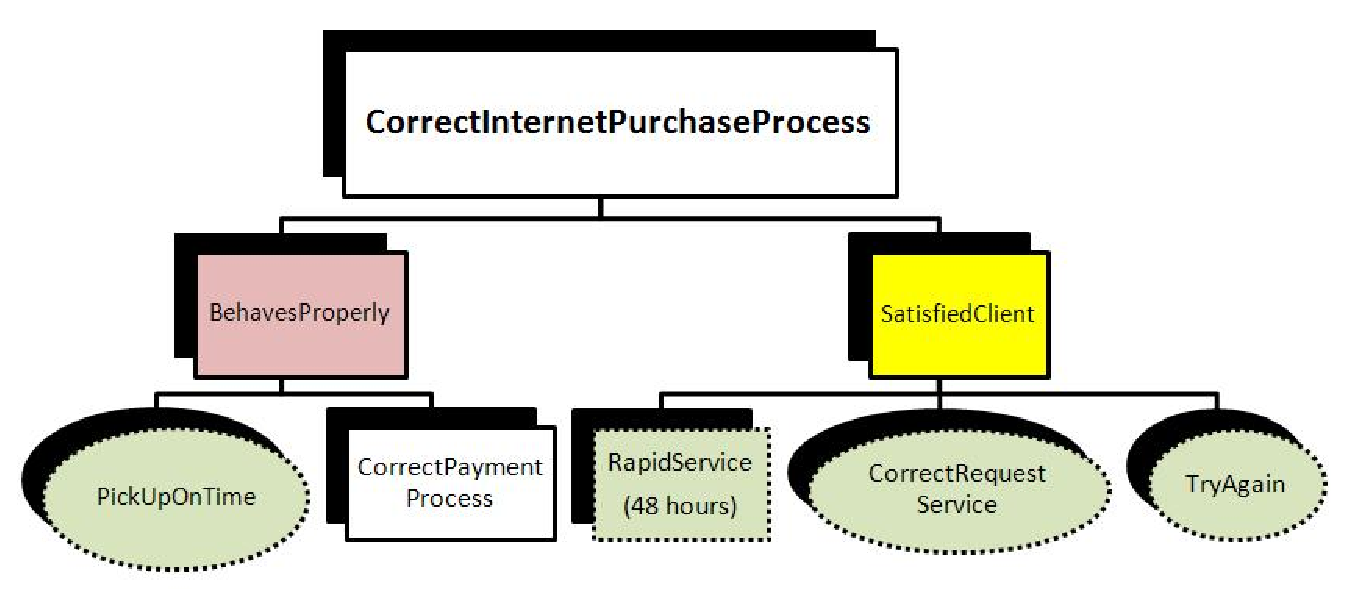
\psfig{file=Figures/InternetPurchaseGoalModel.eps,scale=.60}
%\end{center}
%\caption{The goal-model for the Internet Purchase Process.}
%\label{InternetPurchaseGoalModel}
%\end{figure}
%
%\begin{itemize}
%\item The first subgoal, \emph{``BehavesProperly''}, which is of the ``maintain'' type, is refined by another {\em AND-refinement} with two leaf goals: \emph{``PickupOnTime''}, of ``Unbound Respond'' type, which requires the deliverer to pick up the order on time, otherwise the payment will be refunded, and \emph{``CorrectPaymentProcess''}, of ``maintain'' type, which specifies that the delivery process will not occur if the payment information is not valid.
%%
%\item The second \emph{``SatisfiedClient''}, which is of the ``PossibleAlways'' type, consists of three leaf goals that refine the parent goal by another {\em AND-refinement}: 
%     
%\begin{itemize}
%
%\item \emph{``RapidService''}, of ``Achieve'' type, determines that the client will receive the product on time, that is, within 48 hours after payment.
%
%\item \emph{``CorrectRequestService''}, of ``Unbound Respond'' type, indicates that the product request will only be initiated
%if the product is not out of stock.
%
%\item \emph{``TryAgain"}, of ``Unbound Respond'' type , specifies that the client must be able to repeat the purchase process if the payment is not correct.
%
%\end{itemize}
%
%\end{itemize}
%
%\subsection{Design Phase}\label{PurchaseProcessDesign}
%
%Figure \ref{InternetPurchaseSequenceDiagram} shows the UML 2.0 sequence diagram corresponding to the case study created with the WST tool. In this snapshot we can see the three parties involved in this system with two alt-labelled frames below. The first one captures the possibility of sending correct or incorrect payment information. The second one tests a Boolean variable called ``ValidPayment''. Thus, when the payment information is valid, the Supplier contacts with the Deliverer, who must send the product within the stipulated time. When the payment information is not valid, the Supplier sends a notification to the Client.
%
%\begin{figure}[h]
%\begin{center}
%\psfig{file=Figures/InternetPurchaseSequenceDiagram.eps,scale=.60}
%\end{center}
%\caption{UML 2.0 sequence diagram for the Internet Purchase Process.}
%\label{InternetPurchaseSequenceDiagram}
%\end{figure}
%
%We can also see in the snapshot two exception frames at the end of the diagram. The first one sends a notification to the Client
%when the Supplier is out of stock. The other exception frame states the refund of the payment if the product has not been delivered in the stipulated time.
%
%\subsection{Choreography Implementation Phase}\label{PurchaseProcessChoreography}
%
%First, we export the modelled UML 2.0 sequence diagram to XMI format by using the \textbf{Export XMI} button in the first tab of the WST tool.
%
%Next, we obtain the corresponding WS-CDL code by applying the translation rules introduced in Section \ref{UML2WSCDL}. The second tab of the WST tool is used for this purpose.
%
%A piece of the WS-CDL code generated automatically by the tool can be seen in Figure \ref{codigoWscdl}.
%
%\begin{figure}
%\begin{center}
%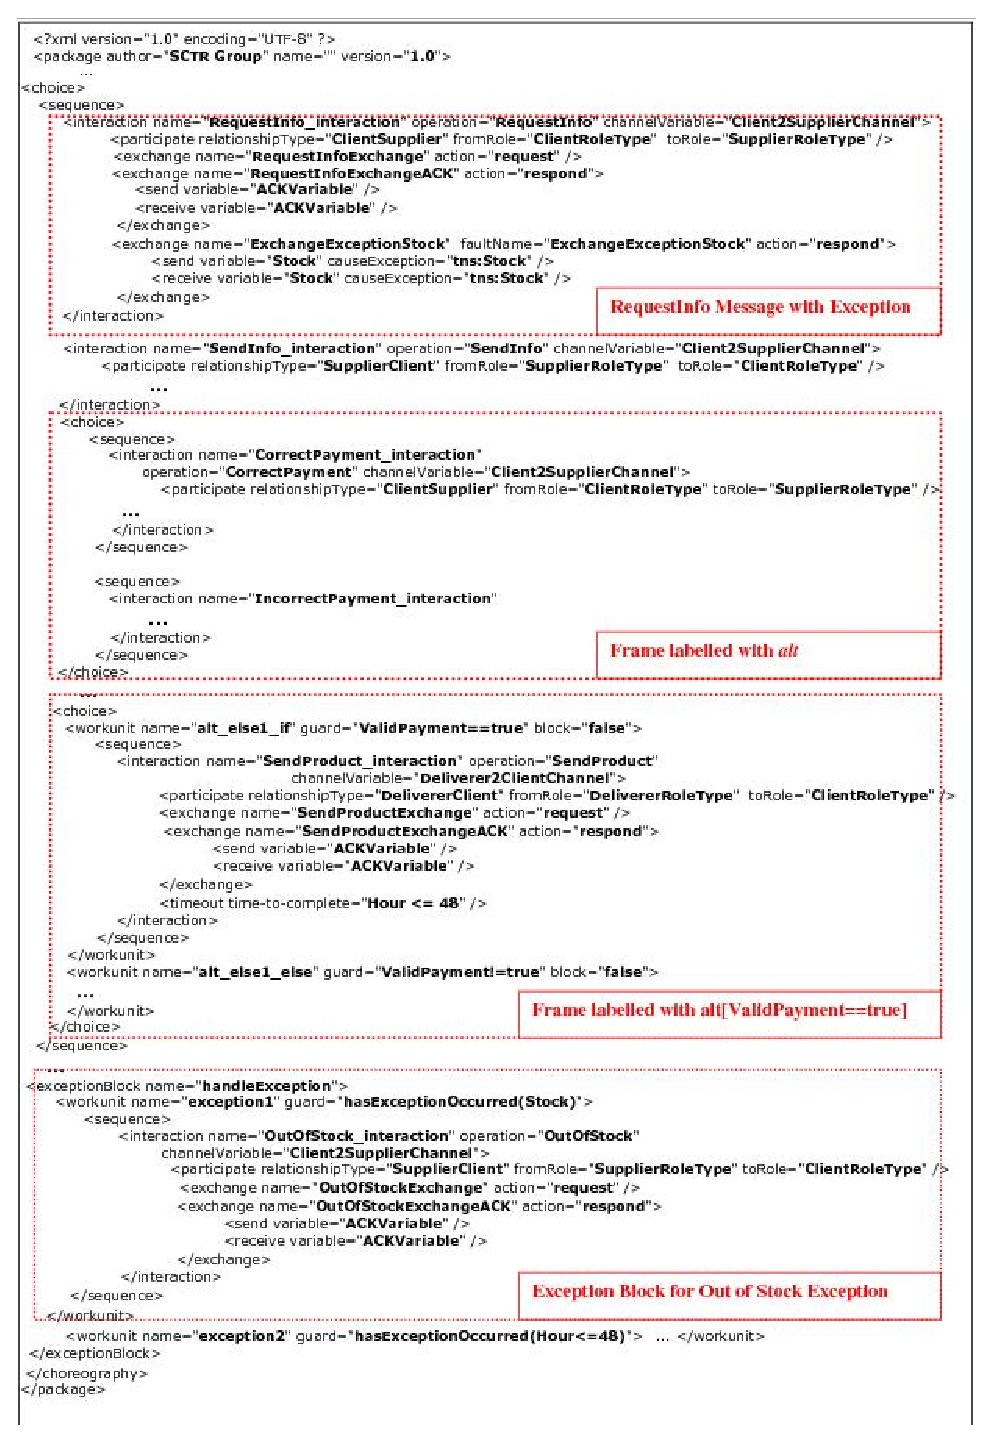
\psfig{file=Figures/codigoWscdl.eps,scale=.80}
%\end{center}
%\caption{A piece of the Internet Purchase Process WS-CDL code.}
%\label{codigoWscdl}
%\end{figure}
%
%\subsection{Verification of Choreography Implementation Phase}\label{PurchaseProcessVerification}
%
%The WS-CDL code we have generated in the previous phase can now be translated into an NTA by following the translation rules introduced in Section \ref{WSCDL2TA}. The third tab of the WST tool is used for this purpose.
%
%The NTA generated automatically by the WST tool for this case study is shown in Figure \ref{InternetPurchaseAutomata}. These automata can be opened by the UPPAAL tool for simulation and verification of properties.
%
%\begin{figure}[h]
%\begin{center}
%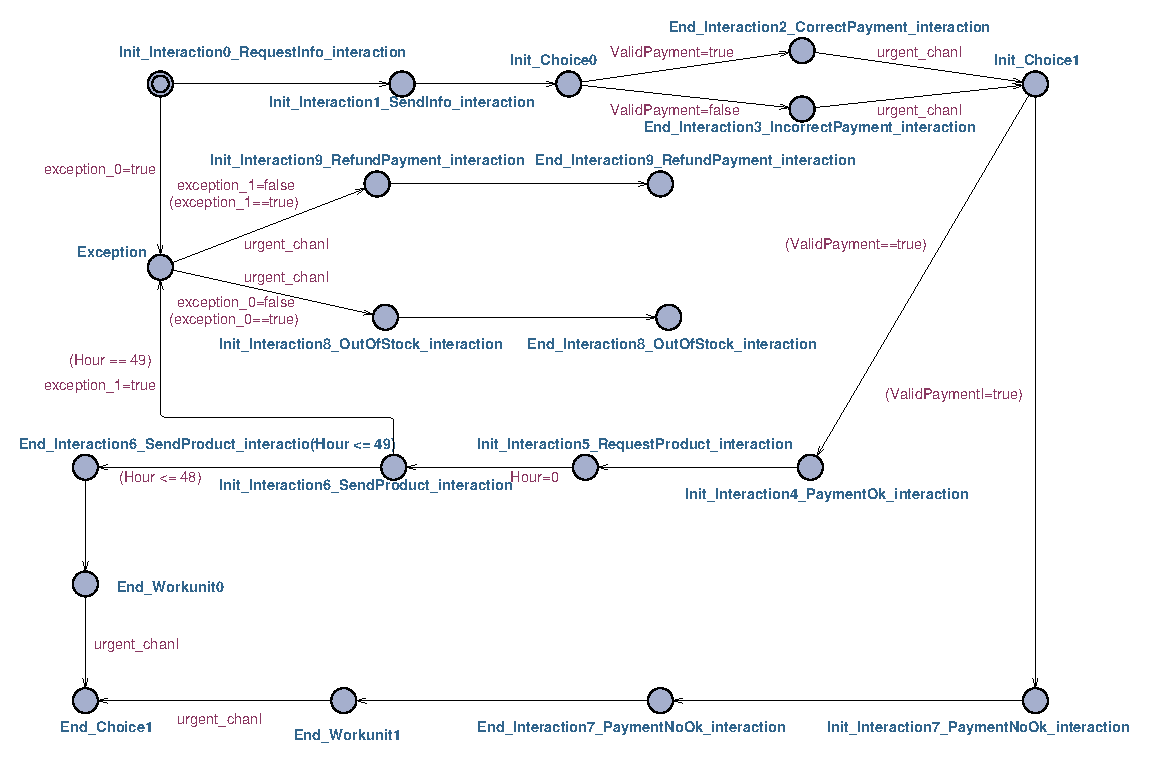
\psfig{file=Figures/InternetPurchaseAutomata.eps,scale=.75}
%\end{center}
%\caption{NTA obtained for the Internet Purchase Process.}
%\label{InternetPurchaseAutomata}
%\end{figure}
%
%In the simulation we check that the system behaves as expected in normal conditions. For this purpose we use the UPPAAL simulator, which can be used in three different ways:
%
%\begin{itemize}
%
%\item The system can be run manually, selecting the transitions to be executed  at each step. 
%
%\item The system can run on its own and the transitions to be performed are therefore selected randomly.
%
%\item The user can run a trace extracted from the verifier. This is usually done in the event of a failure when testing a property, in order to analyze the trace that the verifier provides us, which leads to the state at which the property does not hold.
%
%\end{itemize}
%
%Figure \ref{InternetPurchaseSimulation} depicts a snapshot of the UPPAAL simulator in which we can see one possible simulation of the Internet Purchase Process. 
%
%\begin{figure}[h]
%\begin{center}
%\psfig{file=Figures/InternetPurchaseSimulation.eps,scale=.40}
%\end{center}
%\caption{Simulation of the Internet Purchase Process.}
%\label{InternetPurchaseSimulation}
%\end{figure}
%
%Concerning the verification of properties, we check the properties we have identified in the analysis phase, that is, the leaf goals of the KAOS goal model for the Internet Purchase Process. The correspondence between these goals and the properties we check in the UPPAAL tool is the following:
%
%\begin{itemize}
%
%\item The first leaf goal, \emph{``PickupOnTime''}, specifies that the deliverer must pick up the order on time, i.e., it cannot take more than 48 hours after receiving the request, or an exception will be thrown and the payment will be refunded. This property can be written as follows:
%
%{\normalsize
%\begin{center}
%$(System.Init\_Interaction6\_SendProduct\_interaction \wedge Hour > 48) -->$ $System.Init\_Interaction9\_RefundPayment\_interaction$
%\end{center}
%}
%
%We obtain that this formula is \textbf{satisfied}.
%
%\item The second leaf goal, \emph{``CorrectPaymentProcess''}, specifies that the product will not be delivered if the payment information is not valid. This property is written as follows:
%
%{\normalsize
%\begin{center}
%$A[] \quad ValidPayment==false \quad imply$
%$not \quad System.Init\_Interaction5\_RequestProduct\_interaction$
%\end{center}
%}
%
%We obtain that this formula is \textbf{satisfied}.
%
%\item The third leaf goal, \emph{``RapidService''}, establishes that the client can receive the product on time. This property is written as follows:
%
%{\normalsize
%\begin{center}
%$E<> \quad (System.End\_Interaction6\_SendProduct\_interaction \wedge Hour < 48)$
%\end{center}
%}
%
%We obtain that this formula is \textbf{satisfied}.
%
%\item The fourth leaf goal, \emph{``CorrectRequestService''}, specifies that the purchase process will only be initiated if the product is not out of stock. This property is specified as follows:
%
%{\normalsize
%\begin{center}
%$System.End\_Interaction8\_OutOfStock\_interaction --> not \quad System.Init\_Interaction1\_SendInfo\_interaction$
%\end{center}
%}
%
%We obtain that this formula is also \textbf{satisfied}.
%
%\item The last leaf goal, \emph{``TryAgain''}, specifies that the client must be able to repeat the purchase process if the payment is not correct. This property is written as follows:
%
%{\normalsize
%\begin{center}
%$System.End\_Interaction7\_PaymentNoOk\_interaction --> System.Init\_Interaction1\_SendInfo\_interaction$
%\end{center}
%}
%
%We now obtain that this formula is \textbf{not satisfied}.
%
%\end{itemize}
%
%At this point we have found an error in our design, so we have to go back to the design phase and fix the problem in the UML 2.0 sequence diagram we have modelled. 
%
%In this case study the error found can be easily solved by adding a loop-labelled frame in the diagram wrapping all the payment process and allowing the repetition of the process until the payment is done correctly by establishing a repeat condition.
%
%Once we have done this modification in the sequence diagram designed, all the phases after the design phase must be performed again, that is, the translation of the sequence diagram into a WS-CDL specification, the translation of the WS-CDL specification into timed automata, and the verification of the properties identified in the analysis phase.
%
%After checking all the properties again, we obtain that now all of them are satisfied. Therefore, we do not have to go back to the design phase one more time as all the properties we wanted to check have been satisfied.
%
%This fact does not mean that the implementation of the system is going to be free of error, but we have found and corrected a design error which correction after the implementation of the system would have been much more costly. 
%
%\section{Other Phases of the \textit{Correct-WS} Methodology}\label{OtherPhases}
%\markright{~\ref{OtherPhases} Other Phases of the \textit{Correct-WS} Methodology}
%
%Until now we have seen in detail the phases of the \textit{Correct-WS} methodology automated by the WST tool (Figure \ref{WST_Schema}), that is:
%
%\begin{figure}[h]
%\begin{center}
%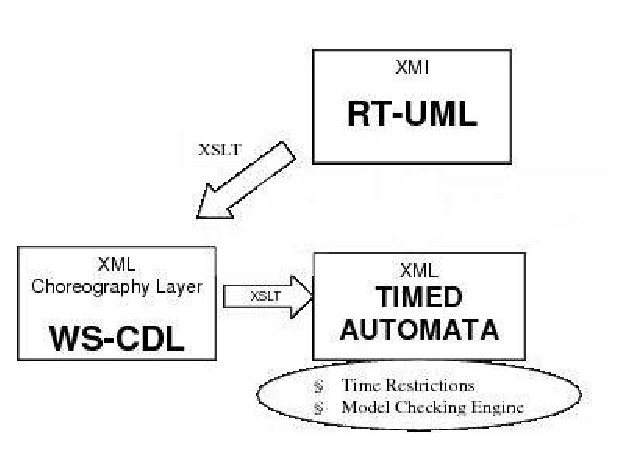
\psfig{file=Figures/WST_Schema.eps,scale=.95}
%\end{center}
%\caption{Scheme of the WST tool translations.}
%\label{WST_Schema}
%\end{figure}
%
%\begin{itemize}
%
%\item The use of UML 2.0 sequence diagrams in order to design the behaviour of the system in a proper way (\textbf{Design phase}).
%
%\item The translation of the UML 2.0 sequence diagrams into a choreography document written in WS-CDL (\textbf{Choreography implementation phase}, not considering the translation into WS-BPEL).
%
%\item The translation of the generated WS-CDL documents into timed automata and the use of the UPPAAL tool in order to check properties, going back to the design phase if failures are found (\textbf{Verification of choreography implementation phase}).
%
%\end{itemize}
%
%We have also depicted the use of KAOS goal models to perform requirement engineering in order to capture the requirements that the system must fulfil (\textbf{Analysis phase}), which integration inside the WST tool is currently under development.
%
%The remaining phases of the \textit{Correct-WS} methodology are covered by several parallel works, some of them briefly described in the following paragraphs.
%
%\textbf{\subsubsection{Translation of UML 2.0 Sequence Diagram into Timed Automata}}
%
%This translation is included in the \textbf{verification of the design phase} of the methodology. In \cite{Cambronero2007} we can find a first approach to an algorithm for this translation, showing its application to an aero-electric management system case study. This algorithm is described in detail in \cite{Cambronero2009}, including its application to some other case studies, such as a travel reservation system and a Internet purchase process.
%
%\textbf{\subsubsection{Translation of UML 2.0 Sequence Diagram into WS-BPEL}}
%
%This translation is an alternative in the \textbf{choreography implementation phase} of the methodology, generating WS-BPEL orchestrations instead of WS-CDL choreographies. We can find a first approach to an algorithm for this translation in \cite{Cambronero2007} and its application to an efficient power production management system case study. The description of the algorithm can also be found in \cite{Cambronero2006} and \cite{Cambronero2007-2}.
%
%\textbf{\subsubsection{Translation of Timed Automata into WS-BPEL}}
%
%This translation is mentioned as a possibility in the \textbf{verification of orchestration implementation phase} of the methodology. In \cite{Cambronero2006} we can find a brief description of this translation.
%
%\textbf{\subsubsection{Translation of WS-BPEL into Timed Automata}}
%
%This translation is also included in the \textbf{verification of orchestration implementation phase} of the methodology. There are many works in the literature focused on this translation \cite{Nakajima2005,Pu2006,Qian2007}, some of them including tool support, so we have not expent additional effort on the development of a new translation from WS-BPEL to timed automata.
%
%\section{Additional Work for Correct Web Services Development}\label{OtherWork}
%\markright{~\ref{OtherWork} Additional Work for Correct Web Services}
%
%Apart from the previous works, all of them included as part of the \textit{Correct-WS} methodology, there are other additional works which aim is also the creation of correct Web Service compositions but are not included as part of the methodology. Anyway, as the goal of these works is actually the same, they are briefly described in the following lines.
%
%\textbf{\subsubsection{Translation of WS-CDL into Coloured Petri Nets}}
%
%Alternatively to the translation of WS-CDL specifications into timed automata, these specifications can be translated to a different formalism and the translation into Coloured Petri nets \cite{Jensen1990} has been proposed. In \cite{Valero2009} an operational semantics and a Petri net semantics are provided for a relevant subset of WS-CDL. In \cite{Valero2009-2} this semantics is extended with time issues and priorities.
%
%\textbf{\subsubsection{Choreography-Conforming Web Service Compositions}}
%
%A formal model, based on finite state machines (FSMs), for defining choreographies and orchestrations is provided in \cite{Diaz2009}. Considering this model, a formal method to derive a set of Web Services from a given choreography, in such a way that the system consisting of these services necessarily conforms to the choreography, is also presented. In \cite{Andres2009} this formal model is extended with priorities to solve the non-determinism problem. A tool to automatically derive choreography-conforming service compositions based on this formal model is currently under development. This tool use a WS-CDL document to specify the choreography, automatically extracting the particular behaviour of each participant in WS-BPEL documents.
%
%\section{Summary}\label{sumWebServ}
%\markright{~\ref{sumWebServ} Summary}
%
%This chapter has described a methodology called \textit{Correct-WS} for the design and verification of Web Service compositions and a tool called WST supporting several phases of this methodology. As a proof of concept the tool has been apply to an Internet purchase process case study. The chapter ends with a brief description of some parallel works which aim is also the development of correct Web Service compositions.
%
%Although in this chapter sequence diagrams have been used to design the service composition behaviour in a proper way, sometimes we just have an electronic contract defining all the contractually correct behaviours of the system in a more general way. In these cases we would like to have a user-friendly representation of the e-contracts but having at the same time a formal background allowing us to verify the correctness of the e-contracts. That is what Chapter \ref{c4} is focused on.